% Options for packages loaded elsewhere
\PassOptionsToPackage{unicode}{hyperref}
\PassOptionsToPackage{hyphens}{url}
%
\documentclass[
]{article}
\usepackage{amsmath,amssymb}
\usepackage{lmodern}
\usepackage{iftex}
\ifPDFTeX
  \usepackage[T1]{fontenc}
  \usepackage[utf8]{inputenc}
  \usepackage{textcomp} % provide euro and other symbols
\else % if luatex or xetex
  \usepackage{unicode-math}
  \defaultfontfeatures{Scale=MatchLowercase}
  \defaultfontfeatures[\rmfamily]{Ligatures=TeX,Scale=1}
\fi
% Use upquote if available, for straight quotes in verbatim environments
\IfFileExists{upquote.sty}{\usepackage{upquote}}{}
\IfFileExists{microtype.sty}{% use microtype if available
  \usepackage[]{microtype}
  \UseMicrotypeSet[protrusion]{basicmath} % disable protrusion for tt fonts
}{}
\makeatletter
\@ifundefined{KOMAClassName}{% if non-KOMA class
  \IfFileExists{parskip.sty}{%
    \usepackage{parskip}
  }{% else
    \setlength{\parindent}{0pt}
    \setlength{\parskip}{6pt plus 2pt minus 1pt}}
}{% if KOMA class
  \KOMAoptions{parskip=half}}
\makeatother
\usepackage{xcolor}
\usepackage[margin=1in]{geometry}
\usepackage{color}
\usepackage{fancyvrb}
\newcommand{\VerbBar}{|}
\newcommand{\VERB}{\Verb[commandchars=\\\{\}]}
\DefineVerbatimEnvironment{Highlighting}{Verbatim}{commandchars=\\\{\}}
% Add ',fontsize=\small' for more characters per line
\usepackage{framed}
\definecolor{shadecolor}{RGB}{248,248,248}
\newenvironment{Shaded}{\begin{snugshade}}{\end{snugshade}}
\newcommand{\AlertTok}[1]{\textcolor[rgb]{0.94,0.16,0.16}{#1}}
\newcommand{\AnnotationTok}[1]{\textcolor[rgb]{0.56,0.35,0.01}{\textbf{\textit{#1}}}}
\newcommand{\AttributeTok}[1]{\textcolor[rgb]{0.77,0.63,0.00}{#1}}
\newcommand{\BaseNTok}[1]{\textcolor[rgb]{0.00,0.00,0.81}{#1}}
\newcommand{\BuiltInTok}[1]{#1}
\newcommand{\CharTok}[1]{\textcolor[rgb]{0.31,0.60,0.02}{#1}}
\newcommand{\CommentTok}[1]{\textcolor[rgb]{0.56,0.35,0.01}{\textit{#1}}}
\newcommand{\CommentVarTok}[1]{\textcolor[rgb]{0.56,0.35,0.01}{\textbf{\textit{#1}}}}
\newcommand{\ConstantTok}[1]{\textcolor[rgb]{0.00,0.00,0.00}{#1}}
\newcommand{\ControlFlowTok}[1]{\textcolor[rgb]{0.13,0.29,0.53}{\textbf{#1}}}
\newcommand{\DataTypeTok}[1]{\textcolor[rgb]{0.13,0.29,0.53}{#1}}
\newcommand{\DecValTok}[1]{\textcolor[rgb]{0.00,0.00,0.81}{#1}}
\newcommand{\DocumentationTok}[1]{\textcolor[rgb]{0.56,0.35,0.01}{\textbf{\textit{#1}}}}
\newcommand{\ErrorTok}[1]{\textcolor[rgb]{0.64,0.00,0.00}{\textbf{#1}}}
\newcommand{\ExtensionTok}[1]{#1}
\newcommand{\FloatTok}[1]{\textcolor[rgb]{0.00,0.00,0.81}{#1}}
\newcommand{\FunctionTok}[1]{\textcolor[rgb]{0.00,0.00,0.00}{#1}}
\newcommand{\ImportTok}[1]{#1}
\newcommand{\InformationTok}[1]{\textcolor[rgb]{0.56,0.35,0.01}{\textbf{\textit{#1}}}}
\newcommand{\KeywordTok}[1]{\textcolor[rgb]{0.13,0.29,0.53}{\textbf{#1}}}
\newcommand{\NormalTok}[1]{#1}
\newcommand{\OperatorTok}[1]{\textcolor[rgb]{0.81,0.36,0.00}{\textbf{#1}}}
\newcommand{\OtherTok}[1]{\textcolor[rgb]{0.56,0.35,0.01}{#1}}
\newcommand{\PreprocessorTok}[1]{\textcolor[rgb]{0.56,0.35,0.01}{\textit{#1}}}
\newcommand{\RegionMarkerTok}[1]{#1}
\newcommand{\SpecialCharTok}[1]{\textcolor[rgb]{0.00,0.00,0.00}{#1}}
\newcommand{\SpecialStringTok}[1]{\textcolor[rgb]{0.31,0.60,0.02}{#1}}
\newcommand{\StringTok}[1]{\textcolor[rgb]{0.31,0.60,0.02}{#1}}
\newcommand{\VariableTok}[1]{\textcolor[rgb]{0.00,0.00,0.00}{#1}}
\newcommand{\VerbatimStringTok}[1]{\textcolor[rgb]{0.31,0.60,0.02}{#1}}
\newcommand{\WarningTok}[1]{\textcolor[rgb]{0.56,0.35,0.01}{\textbf{\textit{#1}}}}
\usepackage{graphicx}
\makeatletter
\def\maxwidth{\ifdim\Gin@nat@width>\linewidth\linewidth\else\Gin@nat@width\fi}
\def\maxheight{\ifdim\Gin@nat@height>\textheight\textheight\else\Gin@nat@height\fi}
\makeatother
% Scale images if necessary, so that they will not overflow the page
% margins by default, and it is still possible to overwrite the defaults
% using explicit options in \includegraphics[width, height, ...]{}
\setkeys{Gin}{width=\maxwidth,height=\maxheight,keepaspectratio}
% Set default figure placement to htbp
\makeatletter
\def\fps@figure{htbp}
\makeatother
\setlength{\emergencystretch}{3em} % prevent overfull lines
\providecommand{\tightlist}{%
  \setlength{\itemsep}{0pt}\setlength{\parskip}{0pt}}
\setcounter{secnumdepth}{-\maxdimen} % remove section numbering
\ifLuaTeX
  \usepackage{selnolig}  % disable illegal ligatures
\fi
\IfFileExists{bookmark.sty}{\usepackage{bookmark}}{\usepackage{hyperref}}
\IfFileExists{xurl.sty}{\usepackage{xurl}}{} % add URL line breaks if available
\urlstyle{same} % disable monospaced font for URLs
\hypersetup{
  pdftitle={9.Random Forest on Lab data -genes},
  pdfauthor={Fay},
  hidelinks,
  pdfcreator={LaTeX via pandoc}}

\title{9.Random Forest on Lab data -genes}
\author{Fay}
\date{2022-11-04}

\begin{document}
\maketitle

\begin{center}\rule{0.5\linewidth}{0.5pt}\end{center}

\hypertarget{aim}{%
\section{Aim:}\label{aim}}

\begin{itemize}
\tightlist
\item
  Predicting health impact of infections utilizing immune parameters as
  predictors
\item
  Predicted variable: WL as a proxy of health
\item
  To do that we are using immune data from experimental lab infections.
\item
  We are training random forest models on the immune data from
  experimental lab infections
\item
  And we test them on the field.
\item
  We then compare the differences in the predicted health impact among
  non-hybrid and hybrid mice.
\end{itemize}

In this document I am preparing the models using the lab data only.

\hypertarget{load-necessary-libraries}{%
\section{Load necessary libraries:}\label{load-necessary-libraries}}

\begin{Shaded}
\begin{Highlighting}[]
\CommentTok{\#install.packages("optimx", version = "2021{-}10.12") \# this package is required for }
\CommentTok{\#the parasite load package to work}
\FunctionTok{library}\NormalTok{(tidyverse)}
\end{Highlighting}
\end{Shaded}

\begin{verbatim}
## Warning: package 'tidyverse' was built under R version 4.2.1
\end{verbatim}

\begin{verbatim}
## Warning: package 'tibble' was built under R version 4.2.1
\end{verbatim}

\begin{verbatim}
## Warning: package 'tidyr' was built under R version 4.2.1
\end{verbatim}

\begin{verbatim}
## Warning: package 'readr' was built under R version 4.2.1
\end{verbatim}

\begin{verbatim}
## Warning: package 'purrr' was built under R version 4.2.1
\end{verbatim}

\begin{verbatim}
## Warning: package 'dplyr' was built under R version 4.2.1
\end{verbatim}

\begin{verbatim}
## Warning: package 'stringr' was built under R version 4.2.2
\end{verbatim}

\begin{verbatim}
## Warning: package 'forcats' was built under R version 4.2.1
\end{verbatim}

\begin{Shaded}
\begin{Highlighting}[]
\FunctionTok{library}\NormalTok{(tidyr)}
\FunctionTok{library}\NormalTok{(dplyr)}
\FunctionTok{library}\NormalTok{(cowplot)}
\FunctionTok{library}\NormalTok{(randomForest)}
\FunctionTok{library}\NormalTok{(ggplot2)}
\FunctionTok{library}\NormalTok{(caret)}
\end{Highlighting}
\end{Shaded}

\begin{verbatim}
## Warning: package 'caret' was built under R version 4.2.1
\end{verbatim}

\begin{Shaded}
\begin{Highlighting}[]
\FunctionTok{library}\NormalTok{(ggpubr)}
\FunctionTok{library}\NormalTok{(rfUtilities) }\CommentTok{\# Implements a permutation test cross{-}validation for }
\end{Highlighting}
\end{Shaded}

\begin{verbatim}
## Warning: package 'rfUtilities' was built under R version 4.2.2
\end{verbatim}

\begin{Shaded}
\begin{Highlighting}[]
\CommentTok{\# Random Forests models}
\end{Highlighting}
\end{Shaded}

\hypertarget{laboratory-data}{%
\section{Laboratory data}\label{laboratory-data}}

\hypertarget{importing-the-data}{%
\subsection{Importing the data}\label{importing-the-data}}

We start with the data from experimental lab infections.

\begin{Shaded}
\begin{Highlighting}[]
\CommentTok{\#import data}
\NormalTok{hm }\OtherTok{\textless{}{-}} \FunctionTok{read.csv}\NormalTok{(}\StringTok{"output\_data/2.imputed\_MICE\_data\_set.csv"}\NormalTok{)}
\end{Highlighting}
\end{Shaded}

\hypertarget{vectors-for-selecting}{%
\section{vectors for selecting}\label{vectors-for-selecting}}

\begin{Shaded}
\begin{Highlighting}[]
\NormalTok{Gene\_lab   }\OtherTok{\textless{}{-}} \FunctionTok{c}\NormalTok{(}\StringTok{"IFNy"}\NormalTok{, }\StringTok{"CXCR3"}\NormalTok{, }\StringTok{"IL.6"}\NormalTok{, }\StringTok{"IL.13"}\NormalTok{, }\CommentTok{\#"IL.10",}
                \StringTok{"IL1RN"}\NormalTok{,}\StringTok{"CASP1"}\NormalTok{, }\StringTok{"CXCL9"}\NormalTok{, }\StringTok{"IDO1"}\NormalTok{, }\StringTok{"IRGM1"}\NormalTok{, }\StringTok{"MPO"}\NormalTok{, }
                \StringTok{"MUC2"}\NormalTok{, }\StringTok{"MUC5AC"}\NormalTok{, }\StringTok{"MYD88"}\NormalTok{, }\StringTok{"NCR1"}\NormalTok{, }\StringTok{"PRF1"}\NormalTok{, }\StringTok{"RETNLB"}\NormalTok{, }\StringTok{"SOCS1"}\NormalTok{, }
                \StringTok{"TICAM1"}\NormalTok{, }\StringTok{"TNF"}\NormalTok{) }\CommentTok{\#"IL.12", "IRG6")}



\NormalTok{Genes\_wild   }\OtherTok{\textless{}{-}} \FunctionTok{c}\NormalTok{(}\StringTok{"IFNy"}\NormalTok{, }\StringTok{"CXCR3"}\NormalTok{, }\StringTok{"IL.6"}\NormalTok{, }\StringTok{"IL.13"}\NormalTok{, }\CommentTok{\#"IL.10", }
                  \StringTok{"IL1RN"}\NormalTok{,}\StringTok{"CASP1"}\NormalTok{, }\StringTok{"CXCL9"}\NormalTok{, }\StringTok{"IDO1"}\NormalTok{, }\StringTok{"IRGM1"}\NormalTok{, }\StringTok{"MPO"}\NormalTok{, }
                  \StringTok{"MUC2"}\NormalTok{, }\StringTok{"MUC5AC"}\NormalTok{, }\StringTok{"MYD88"}\NormalTok{, }\StringTok{"NCR1"}\NormalTok{, }\StringTok{"PRF1"}\NormalTok{, }\StringTok{"RETNLB"}\NormalTok{, }\StringTok{"SOCS1"}\NormalTok{, }
                  \StringTok{"TICAM1"}\NormalTok{, }\StringTok{"TNF"}\NormalTok{) }\CommentTok{\#, "IL.12", "IRG6")}



\NormalTok{Facs\_lab }\OtherTok{\textless{}{-}} \FunctionTok{c}\NormalTok{(}\StringTok{"Position"}\NormalTok{, }\StringTok{"CD4"}\NormalTok{, }\StringTok{"Treg"}\NormalTok{, }\StringTok{"Div\_Treg"}\NormalTok{, }\StringTok{"Treg17"}\NormalTok{, }\StringTok{"Th1"}\NormalTok{, }
                    \StringTok{"Div\_Th1"}\NormalTok{, }\StringTok{"Th17"}\NormalTok{, }\StringTok{"Div\_Th17"}\NormalTok{, }\StringTok{"CD8"}\NormalTok{, }\StringTok{"Act\_CD8"}\NormalTok{, }
                    \StringTok{"Div\_Act\_CD8"}\NormalTok{, }\StringTok{"IFNy\_CD4"}\NormalTok{, }\StringTok{"IFNy\_CD8"}\NormalTok{,}\StringTok{"Treg\_prop"}\NormalTok{, }
                    \StringTok{"IL17A\_CD4"}\NormalTok{)  }

\NormalTok{Facs\_wild }\OtherTok{\textless{}{-}} \FunctionTok{c}\NormalTok{( }\StringTok{"Treg"}\NormalTok{, }\StringTok{"CD4"}\NormalTok{, }\StringTok{"Treg17"}\NormalTok{, }\StringTok{"Th1"}\NormalTok{, }\StringTok{"Th17"}\NormalTok{, }\StringTok{"CD8"}\NormalTok{,}
                     \StringTok{"Act\_CD8"}\NormalTok{, }\StringTok{"IFNy\_CD4"}\NormalTok{, }\StringTok{"IL17A\_CD4"}\NormalTok{, }\StringTok{"IFNy\_CD8"}\NormalTok{)}
\end{Highlighting}
\end{Shaded}

\hypertarget{data-cleaning-preparation}{%
\subsection{Data cleaning /
preparation}\label{data-cleaning-preparation}}

\begin{Shaded}
\begin{Highlighting}[]
\CommentTok{\# we need to change the  in challenge infections to a factor}
\NormalTok{hm}\SpecialCharTok{$}\NormalTok{Parasite\_challenge }\OtherTok{\textless{}{-}} \FunctionTok{as.factor}\NormalTok{(hm}\SpecialCharTok{$}\NormalTok{Parasite\_challenge)}
\NormalTok{hm}\SpecialCharTok{$}\NormalTok{MC.Eimeria }\OtherTok{\textless{}{-}} \FunctionTok{as.factor}\NormalTok{(hm}\SpecialCharTok{$}\NormalTok{MC.Eimeria)}

\CommentTok{\# Here I create a new column, where we get the actual infection status}
\CommentTok{\# According to the melting curve for eimeria }
\NormalTok{hm }\OtherTok{\textless{}{-}}\NormalTok{ hm }\SpecialCharTok{\%\textgreater{}\%}
\NormalTok{  dplyr}\SpecialCharTok{::}\FunctionTok{mutate}\NormalTok{(}\AttributeTok{infection =} \FunctionTok{case\_when}\NormalTok{(}
\NormalTok{    Parasite\_challenge }\SpecialCharTok{==} \StringTok{"E\_ferrisi"} \SpecialCharTok{\&}\NormalTok{ MC.Eimeria }\SpecialCharTok{==} \StringTok{"TRUE"} \SpecialCharTok{\textasciitilde{}} \StringTok{"E\_ferrisi"}\NormalTok{,}
\NormalTok{    Parasite\_challenge }\SpecialCharTok{==} \StringTok{"E\_ferrisi"} \SpecialCharTok{\&}\NormalTok{ MC.Eimeria }\SpecialCharTok{==} \StringTok{"FALSE"} \SpecialCharTok{\textasciitilde{}} \StringTok{"uninfected"}\NormalTok{,}
\NormalTok{    Parasite\_challenge }\SpecialCharTok{==} \StringTok{"E\_falciformis"} \SpecialCharTok{\&}\NormalTok{ MC.Eimeria }\SpecialCharTok{==} \StringTok{"TRUE"} \SpecialCharTok{\textasciitilde{}} \StringTok{"E\_falciformis"}\NormalTok{,}
\NormalTok{    Parasite\_challenge }\SpecialCharTok{==} \StringTok{"E\_falciformis"} \SpecialCharTok{\&}\NormalTok{ MC.Eimeria }\SpecialCharTok{==} \StringTok{"FALSE"} \SpecialCharTok{\textasciitilde{}} \StringTok{"uninfected"}\NormalTok{,}
\NormalTok{    Parasite\_challenge }\SpecialCharTok{==} \StringTok{"uninfected"} \SpecialCharTok{\&}\NormalTok{ MC.Eimeria }\SpecialCharTok{==} \StringTok{"TRUE"} \SpecialCharTok{\textasciitilde{}} \StringTok{"infected\_eimeria"}\NormalTok{,}
\NormalTok{    Parasite\_challenge }\SpecialCharTok{==} \StringTok{"uninfected"} \SpecialCharTok{\&}\NormalTok{ MC.Eimeria }\SpecialCharTok{==} \StringTok{"FALSE"} \SpecialCharTok{\textasciitilde{}} \StringTok{"uninfected"}\NormalTok{,}
    \ConstantTok{TRUE} \SpecialCharTok{\textasciitilde{}} \StringTok{""}
\NormalTok{  ))}


\CommentTok{\# Here I create a new column, where we get the actual infection status}
\CommentTok{\# According to the melting curve for eimeria }
\NormalTok{hm }\OtherTok{\textless{}{-}}\NormalTok{ hm }\SpecialCharTok{\%\textgreater{}\%}
\NormalTok{  dplyr}\SpecialCharTok{::}\FunctionTok{mutate}\NormalTok{(}\AttributeTok{infection =} \FunctionTok{case\_when}\NormalTok{(}
\NormalTok{    Parasite\_challenge }\SpecialCharTok{==} \StringTok{"E\_ferrisi"} \SpecialCharTok{\&}\NormalTok{ MC.Eimeria }\SpecialCharTok{==} \StringTok{"TRUE"} \SpecialCharTok{\textasciitilde{}} \StringTok{"E\_ferrisi"}\NormalTok{,}
\NormalTok{    Parasite\_challenge }\SpecialCharTok{==} \StringTok{"E\_ferrisi"} \SpecialCharTok{\&}\NormalTok{ MC.Eimeria }\SpecialCharTok{==} \StringTok{"FALSE"} \SpecialCharTok{\textasciitilde{}} \StringTok{"uninfected"}\NormalTok{,}
\NormalTok{    Parasite\_challenge }\SpecialCharTok{==} \StringTok{"E\_falciformis"} \SpecialCharTok{\&}\NormalTok{ MC.Eimeria }\SpecialCharTok{==} \StringTok{"TRUE"} \SpecialCharTok{\textasciitilde{}} \StringTok{"E\_falciformis"}\NormalTok{,}
\NormalTok{    Parasite\_challenge }\SpecialCharTok{==} \StringTok{"E\_falciformis"} \SpecialCharTok{\&}\NormalTok{ MC.Eimeria }\SpecialCharTok{==} \StringTok{"FALSE"} \SpecialCharTok{\textasciitilde{}} \StringTok{"uninfected"}\NormalTok{,}
\NormalTok{    Parasite\_challenge }\SpecialCharTok{==} \StringTok{"uninfected"} \SpecialCharTok{\&}\NormalTok{ MC.Eimeria }\SpecialCharTok{==} \StringTok{"TRUE"} \SpecialCharTok{\textasciitilde{}} \StringTok{"E\_falciformis"}\NormalTok{,}
\NormalTok{    Parasite\_challenge }\SpecialCharTok{==} \StringTok{"uninfected"} \SpecialCharTok{\&}\NormalTok{ MC.Eimeria }\SpecialCharTok{==} \StringTok{"FALSE"} \SpecialCharTok{\textasciitilde{}} \StringTok{"uninfected"}\NormalTok{,}
    \ConstantTok{TRUE} \SpecialCharTok{\textasciitilde{}} \StringTok{""}
\NormalTok{  ))}
\end{Highlighting}
\end{Shaded}

\hypertarget{splitting-data-into-training-and-testing-sets}{%
\subsection{Splitting data into training and testing
sets}\label{splitting-data-into-training-and-testing-sets}}

Splitting between training and testing: - Assess model performance on
unseen data - Avoid over-fitting

\hypertarget{cross-validation-in-r}{%
\subsection{Cross validation in R}\label{cross-validation-in-r}}

k - fold cross validation: the data set is divided into k subsets. Each
time, one of the k subsets is used as the test set and

\hypertarget{random-forest-for-predicting-percentage-of-maximum-weight-loss}{%
\section{Random forest for predicting percentage of maximum weight
loss}\label{random-forest-for-predicting-percentage-of-maximum-weight-loss}}

\hypertarget{dividing-data-into-training-and-testing}{%
\subsection{Dividing data into training and
testing}\label{dividing-data-into-training-and-testing}}

\begin{Shaded}
\begin{Highlighting}[]
\CommentTok{\# prepare the lab data}
\NormalTok{lab }\OtherTok{\textless{}{-}}\NormalTok{ hm }\SpecialCharTok{\%\textgreater{}\%} 
\NormalTok{  dplyr}\SpecialCharTok{::}\FunctionTok{filter}\NormalTok{(origin }\SpecialCharTok{==} \StringTok{"Lab"}\NormalTok{)}


\CommentTok{\#select the imputed gene columns}
\NormalTok{gene }\OtherTok{\textless{}{-}}\NormalTok{  lab }\SpecialCharTok{\%\textgreater{}\%}
\NormalTok{  dplyr}\SpecialCharTok{::}\FunctionTok{select}\NormalTok{(}\FunctionTok{c}\NormalTok{(Mouse\_ID, }\FunctionTok{all\_of}\NormalTok{(Gene\_lab)))}

\NormalTok{gene }\OtherTok{\textless{}{-}} \FunctionTok{unique}\NormalTok{(gene)}

\NormalTok{genes }\OtherTok{\textless{}{-}}\NormalTok{ gene }\SpecialCharTok{\%\textgreater{}\%}
\NormalTok{  dplyr}\SpecialCharTok{::}\FunctionTok{select}\NormalTok{(}\SpecialCharTok{{-}}\NormalTok{Mouse\_ID)}

\CommentTok{\#remove rows with only nas}
\NormalTok{genes }\OtherTok{\textless{}{-}}\NormalTok{ genes[,}\FunctionTok{colSums}\NormalTok{(}\FunctionTok{is.na}\NormalTok{(genes))}\SpecialCharTok{\textless{}}\FunctionTok{nrow}\NormalTok{(genes)]}

\CommentTok{\#remove colums with only nas }
\NormalTok{genes }\OtherTok{\textless{}{-}}\NormalTok{ genes[}\FunctionTok{rowSums}\NormalTok{(}\FunctionTok{is.na}\NormalTok{(genes)) }\SpecialCharTok{!=} \FunctionTok{ncol}\NormalTok{(genes), ]}

\CommentTok{\# select the same rows from the gene data}
\NormalTok{gene }\OtherTok{\textless{}{-}}\NormalTok{ gene[}\FunctionTok{row.names}\NormalTok{(genes),]}

\CommentTok{\# select the same rows from the lab data}
\NormalTok{lab }\OtherTok{\textless{}{-}}\NormalTok{ lab[}\FunctionTok{row.names}\NormalTok{(genes),]}


\NormalTok{gene }\OtherTok{\textless{}{-}}\NormalTok{ lab }\SpecialCharTok{\%\textgreater{}\%}
\NormalTok{  dplyr}\SpecialCharTok{::}\FunctionTok{select}\NormalTok{(}\FunctionTok{c}\NormalTok{(Mouse\_ID, WL\_max)) }\SpecialCharTok{\%\textgreater{}\%}
  \FunctionTok{right\_join}\NormalTok{(gene, }\AttributeTok{by =} \StringTok{"Mouse\_ID"}\NormalTok{)}

\NormalTok{gene }\OtherTok{\textless{}{-}} \FunctionTok{unique}\NormalTok{(gene) }\SpecialCharTok{\%\textgreater{}\%}
\NormalTok{  dplyr}\SpecialCharTok{::}\FunctionTok{select}\NormalTok{(}\SpecialCharTok{{-}}\NormalTok{Mouse\_ID)}
\end{Highlighting}
\end{Shaded}

\hypertarget{cross-validation}{%
\subsection{Cross validation}\label{cross-validation}}

mtry: Number of variable is randomly collected to be sampled at each
split time ntree: Number of trees you are going to grow in this random
forest

\url{https://rpubs.com/jvaldeleon/forest_repeat_cv}

cross validation

The general procedure is like this.

We shuffle the data by random.

We split it into k-groups. Note that k is an arbitrary parameter.
There's no specific criteria to choose the value for k. Typically, it's
5 or 10.

For each unique group:

\begin{enumerate}
\def\labelenumi{\arabic{enumi}.}
\item
  Take the group as a hold out or test data set
\item
  Take the remaining groups as a training data set
\item
  Fit a model on the training set and evaluate it on the test set
\item
  Retain the evaluation score and discard the model
\end{enumerate}

\begin{Shaded}
\begin{Highlighting}[]
\NormalTok{repeat\_cv }\OtherTok{\textless{}{-}} \FunctionTok{trainControl}\NormalTok{(}\AttributeTok{method =} \StringTok{"repeatedcv"}\NormalTok{, }\CommentTok{\#repeated cross validation}
                           \AttributeTok{number =} \DecValTok{5}\NormalTok{, }\CommentTok{\# 5 fold cross validation}
                           \AttributeTok{repeats =} \DecValTok{3}\NormalTok{)}
\end{Highlighting}
\end{Shaded}

\hypertarget{splitting-into-training-and-testing}{%
\subsection{Splitting into training and
testing}\label{splitting-into-training-and-testing}}

\begin{Shaded}
\begin{Highlighting}[]
\CommentTok{\# split data into training and test}
\FunctionTok{set.seed}\NormalTok{(}\DecValTok{333}\NormalTok{) }\CommentTok{\# this will help us reproduce this random assignment}

\CommentTok{\# in this way we can pick the random numbers}
\NormalTok{training.samples }\OtherTok{\textless{}{-}} \FunctionTok{createDataPartition}\NormalTok{(}\AttributeTok{y =}\NormalTok{ gene}\SpecialCharTok{$}\NormalTok{WL\_max, }\AttributeTok{p =}\NormalTok{ .}\DecValTok{7}\NormalTok{, }\AttributeTok{list =} \ConstantTok{FALSE}\NormalTok{) }

\CommentTok{\# this is the partiicition! In this case 0.7 = training data and 0.3 = testing}
\CommentTok{\# we don\textquotesingle{}t want to get a list in return}
\NormalTok{train.data }\OtherTok{\textless{}{-}}\NormalTok{ gene[training.samples, ] }
\NormalTok{test.data }\OtherTok{\textless{}{-}}\NormalTok{ gene[}\SpecialCharTok{{-}}\NormalTok{training.samples, ] }
\end{Highlighting}
\end{Shaded}

\hypertarget{building-the-model}{%
\subsection{Building the model}\label{building-the-model}}

\begin{Shaded}
\begin{Highlighting}[]
\FunctionTok{set.seed}\NormalTok{(}\DecValTok{333}\NormalTok{)}


\CommentTok{\#train the model}
\NormalTok{WL\_predict\_gene }\OtherTok{\textless{}{-}} \FunctionTok{randomForest}\NormalTok{(WL\_max }\SpecialCharTok{\textasciitilde{}}\NormalTok{., }\AttributeTok{data =}\NormalTok{ train.data, }
                                    \AttributeTok{proximity =} \ConstantTok{TRUE}\NormalTok{, }\AttributeTok{ntree =} \DecValTok{1000}\NormalTok{) }
\CommentTok{\# ntree = number of trees     }
\CommentTok{\# save the model }
\FunctionTok{save}\NormalTok{(WL\_predict\_gene, }\AttributeTok{file =}  \StringTok{"r\_scripts/models/WL\_predict\_gene.RData"}\NormalTok{)}
\FunctionTok{print}\NormalTok{(WL\_predict\_gene)}
\end{Highlighting}
\end{Shaded}

\begin{verbatim}
## 
## Call:
##  randomForest(formula = WL_max ~ ., data = train.data, proximity = TRUE,      ntree = 1000) 
##                Type of random forest: regression
##                      Number of trees: 1000
## No. of variables tried at each split: 6
## 
##           Mean of squared residuals: 37.2864
##                     % Var explained: 38.71
\end{verbatim}

Plotting the WL\_predict\_gene will illustrate the error rate as we
average across more trees and shows that our error rate stabalizes with
around 200 trees.

\hypertarget{model---quality-testing}{%
\subsection{Model - quality testing}\label{model---quality-testing}}

\hypertarget{cross-validation-1}{%
\subsubsection{Cross-validation}\label{cross-validation-1}}

MSE: As a brief explanation, mean squared error (MSE) is the average of
the summation of the squared difference between the actual output value
and the predicted output value. Our goal is to reduce the MSE as much as
possible.

Variance explained: \%explained variance is a measure of how well
out-of-bag predictions explain the target variance of the training set.

\begin{Shaded}
\begin{Highlighting}[]
\NormalTok{predict\_WL\_cv }\OtherTok{\textless{}{-}} \FunctionTok{rf.crossValidation}\NormalTok{(}\AttributeTok{x =}\NormalTok{ WL\_predict\_gene, }\AttributeTok{xdata =}\NormalTok{ train.data, }
                                    \AttributeTok{p =} \FloatTok{0.10}\NormalTok{, }\AttributeTok{n =} \DecValTok{99}\NormalTok{, }\AttributeTok{ntree =} \DecValTok{501}\NormalTok{)}
\end{Highlighting}
\end{Shaded}

\begin{verbatim}
## running: regression cross-validation with 99 iterations
\end{verbatim}

\begin{Shaded}
\begin{Highlighting}[]
\NormalTok{predict\_WL\_cv}\SpecialCharTok{$}\NormalTok{fit.var.exp}
\end{Highlighting}
\end{Shaded}

\begin{verbatim}
## [1] 38.71
\end{verbatim}

\begin{Shaded}
\begin{Highlighting}[]
\FunctionTok{par}\NormalTok{(}\AttributeTok{mfrow=}\FunctionTok{c}\NormalTok{(}\DecValTok{2}\NormalTok{,}\DecValTok{2}\NormalTok{))}

\FunctionTok{plot}\NormalTok{(predict\_WL\_cv) }

\CommentTok{\# Root Mean Squared Error (observed vs. predicted) from each Bootstrap }
\CommentTok{\# iteration (cross{-}validation)}
\FunctionTok{plot}\NormalTok{(predict\_WL\_cv, }\AttributeTok{stat =} \StringTok{"mse"}\NormalTok{)}

\CommentTok{\#Percent variance explained from specified fit model}
\FunctionTok{plot}\NormalTok{(predict\_WL\_cv, }\AttributeTok{stat =} \StringTok{"var.exp"}\NormalTok{)}

\CommentTok{\#Mean Absolute Error from each Bootstrapped model}
\FunctionTok{plot}\NormalTok{(predict\_WL\_cv, }\AttributeTok{stat =} \StringTok{"mae"}\NormalTok{)}
\end{Highlighting}
\end{Shaded}

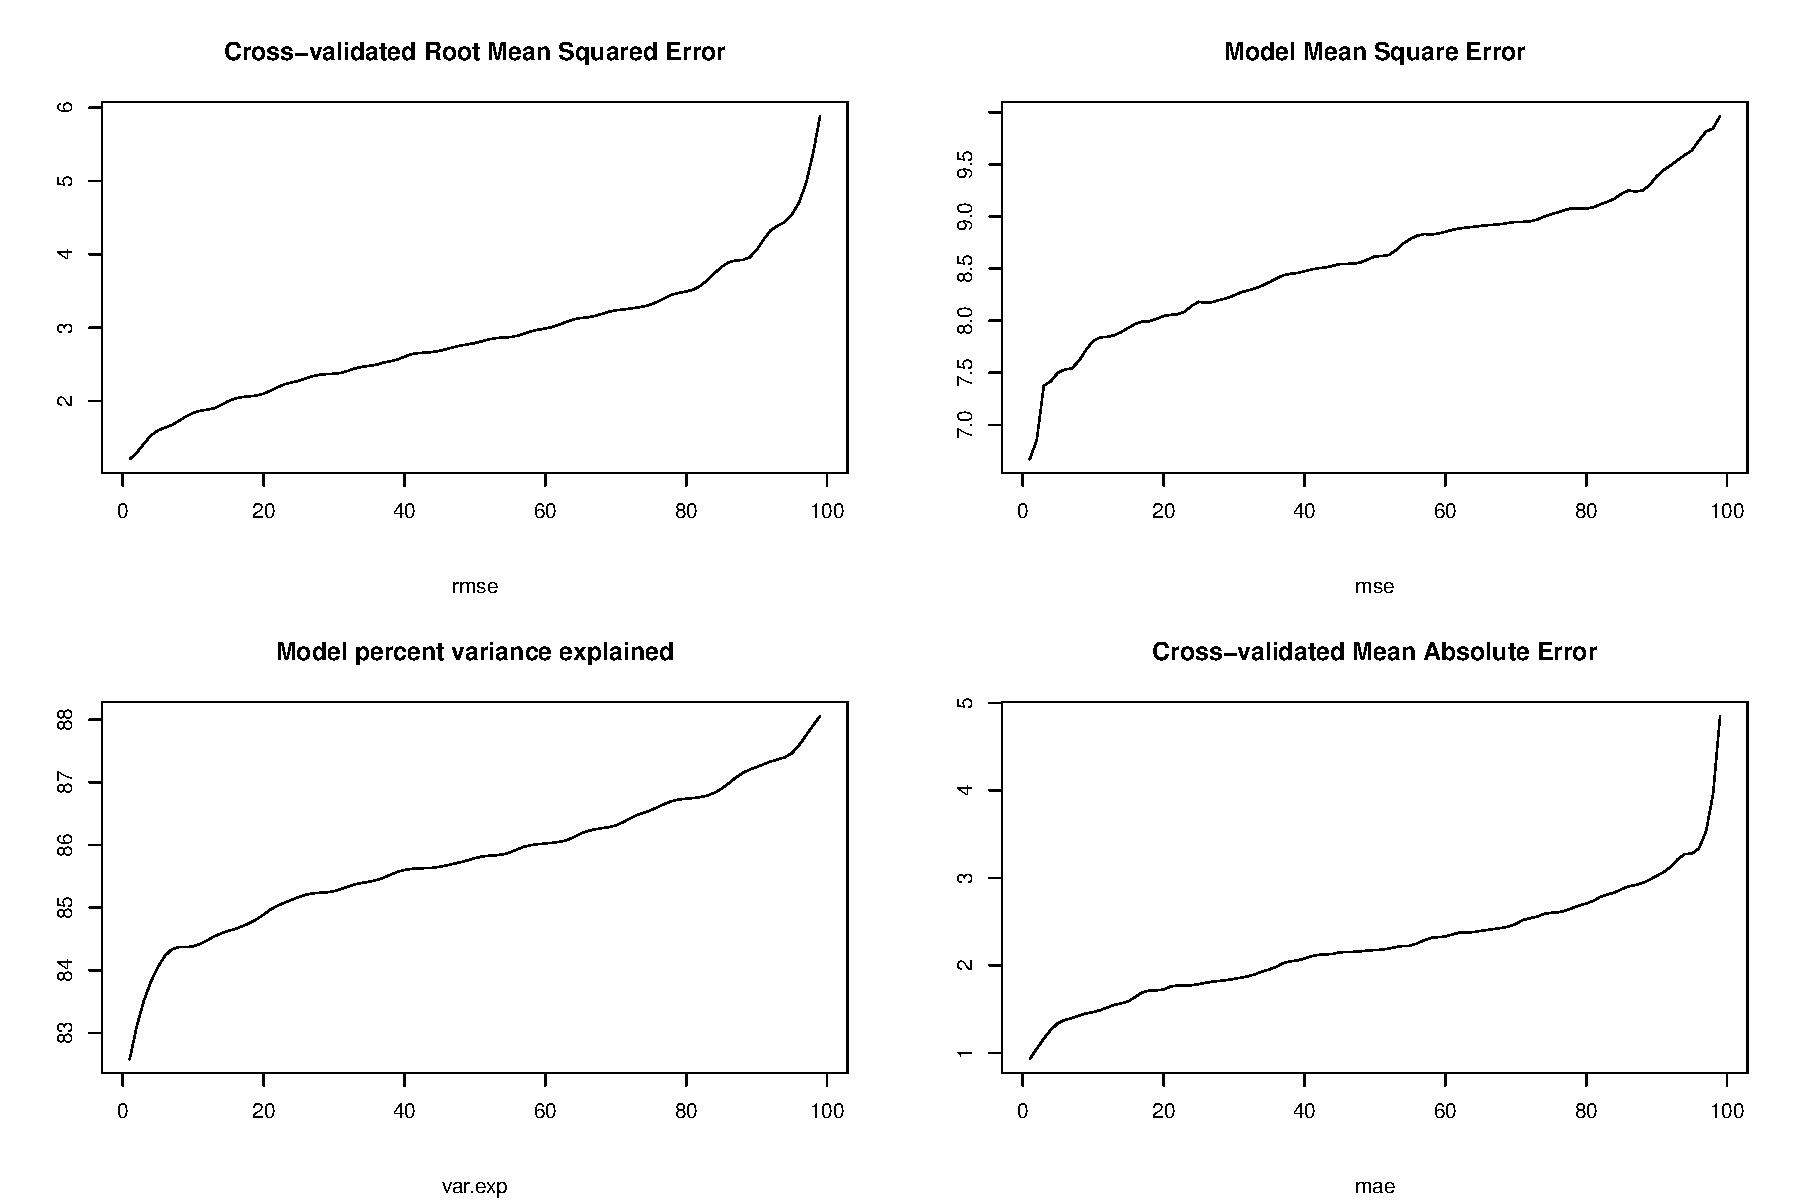
\includegraphics{8.Random_Forest_lab_gene_files/figure-latex/unnamed-chunk-4-1.pdf}

\begin{Shaded}
\begin{Highlighting}[]
\FunctionTok{plot}\NormalTok{(WL\_predict\_gene)}
\end{Highlighting}
\end{Shaded}

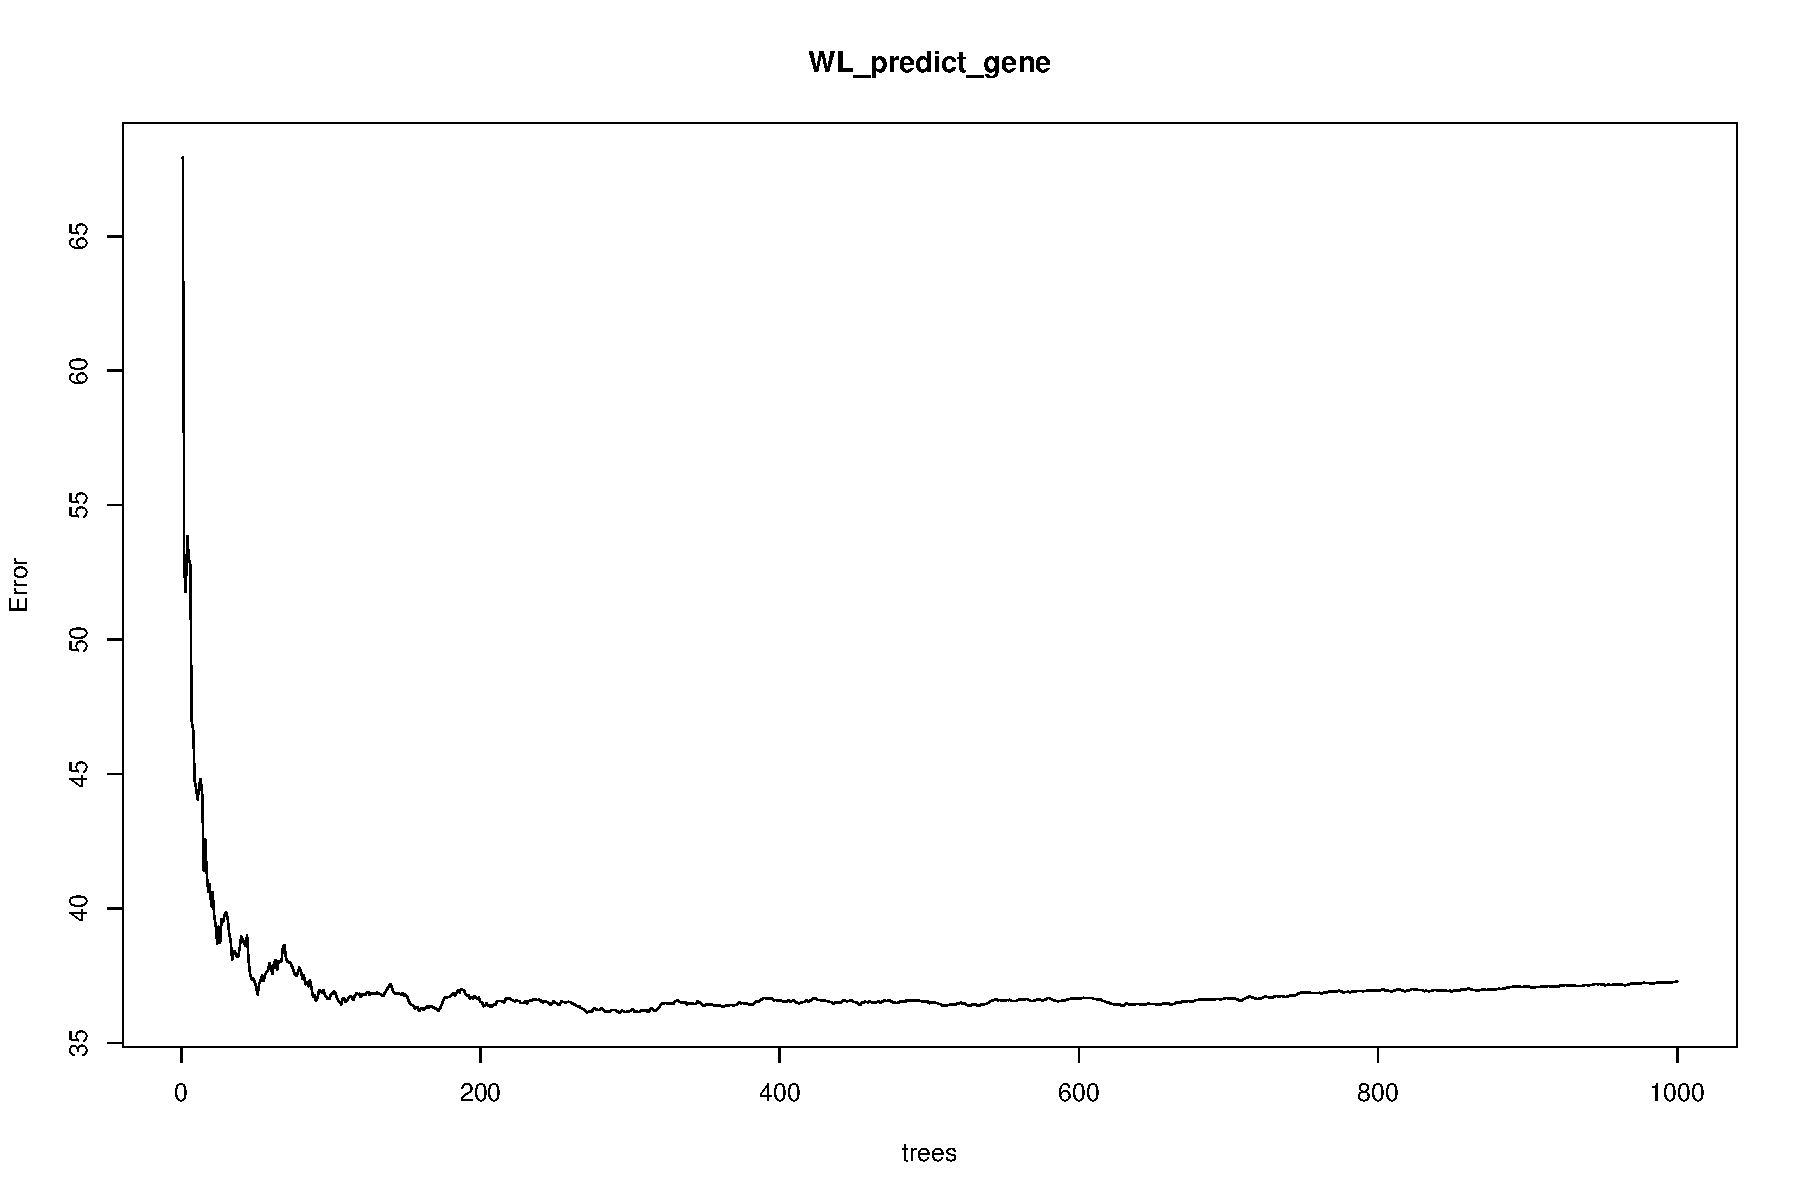
\includegraphics{8.Random_Forest_lab_gene_files/figure-latex/unnamed-chunk-5-1.pdf}
The plotted error rate above is based on the OOB sample error and can be
accessed directly at m1\$mse. Thus, we can find which number of trees
providing the lowest error rate

\begin{Shaded}
\begin{Highlighting}[]
\CommentTok{\# number of trees with lowest MSE}
\FunctionTok{which.min}\NormalTok{(WL\_predict\_gene}\SpecialCharTok{$}\NormalTok{mse)}
\end{Highlighting}
\end{Shaded}

\begin{verbatim}
## [1] 293
\end{verbatim}

\begin{Shaded}
\begin{Highlighting}[]
\CommentTok{\# RMSE of this optimal random forest}
\FunctionTok{sqrt}\NormalTok{(WL\_predict\_gene}\SpecialCharTok{$}\NormalTok{mse[}\FunctionTok{which.min}\NormalTok{(WL\_predict\_gene}\SpecialCharTok{$}\NormalTok{mse)])}
\end{Highlighting}
\end{Shaded}

\begin{verbatim}
## [1] 6.00987
\end{verbatim}

\hypertarget{httpsuc-r.github.ios}{%
\subsubsection{\texorpdfstring{\url{https://uc-r.github.io/s}}{https://uc-r.github.io/s}}\label{httpsuc-r.github.ios}}

RandomForest also allows us to use a validation set to measure
predictive accuracy if we did not want to use the OOB samples.

Tutorial:
\url{https://hackernoon.com/random-forest-regression-in-r-code-and-interpretation}

Random forest regression in R provides two outputs: decrease in mean
square error (MSE) and node purity. Prediction error described as MSE is
based on permuting out-of-bag sections of the data per individual tree
and predictor, and the errors are then averaged. In the regression
context, Node purity is the total decrease in residual sum of squares
when splitting on a variable averaged over all trees (i.e.~how well a
predictor decreases variance). MSE is a more reliable measure of
variable importance. If the two importance metrics show different
results, listen to MSE. If all of your predictors are numerical, then it
shouldn't be too much of an issue

Mean Decrease Gini (IncNodePurity) - This is a measure of variable
importance based on the Gini impurity index used for the calculating the
splits in trees.

Improving Your Model Your model depends on the quality of your dataset
and the type of Machine Learning algorithm used. Therefore, to improve
the accuracy of your model, you should:

Check what attributes affect our model the most and what variables to
leave out in future analysis Find out what other attributes affect a
person's wage; we can use as predictors in future analysis Tweak the
algorithm (e.g.~change the ntree value) Use a different machine learning
algorithm If any of these reduces the RMSE significantly, you have
succeeded in improving your model!

\hypertarget{application-of-wl_predict_gene}{%
\section{Application of
WL\_predict\_gene}\label{application-of-wl_predict_gene}}

\hypertarget{using-the-testing-data}{%
\subsection{Using the testing data}\label{using-the-testing-data}}

Let's now make some predictions using our test data.

\begin{Shaded}
\begin{Highlighting}[]
\CommentTok{\#The predict() function in R is used to predict the values based on the }
\CommentTok{\# input data.}
\NormalTok{predictions }\OtherTok{\textless{}{-}} \FunctionTok{predict}\NormalTok{(WL\_predict\_gene, test.data)}

\CommentTok{\# assign test.data to a new object, so that we can make changes}
\NormalTok{result }\OtherTok{\textless{}{-}}\NormalTok{ test.data}

\CommentTok{\#add the new variable of predictions to the result object}
\NormalTok{result }\OtherTok{\textless{}{-}} \FunctionTok{cbind}\NormalTok{(result, predictions)}

\CommentTok{\# what is the correlation between predicted and actual data?}
\FunctionTok{cor}\NormalTok{(result}\SpecialCharTok{$}\NormalTok{WL\_max, result}\SpecialCharTok{$}\NormalTok{predictions, }
    \AttributeTok{method =} \FunctionTok{c}\NormalTok{(}\StringTok{"pearson"}\NormalTok{, }\StringTok{"kendall"}\NormalTok{, }\StringTok{"spearman"}\NormalTok{))}
\end{Highlighting}
\end{Shaded}

\begin{verbatim}
## [1] 0.8705605
\end{verbatim}

\begin{Shaded}
\begin{Highlighting}[]
\FunctionTok{cor.test}\NormalTok{(result}\SpecialCharTok{$}\NormalTok{WL\_max, result}\SpecialCharTok{$}\NormalTok{predictions)}
\end{Highlighting}
\end{Shaded}

\begin{verbatim}
## 
##  Pearson's product-moment correlation
## 
## data:  result$WL_max and result$predictions
## t = 10.762, df = 37, p-value = 5.975e-13
## alternative hypothesis: true correlation is not equal to 0
## 95 percent confidence interval:
##  0.7652360 0.9304929
## sample estimates:
##       cor 
## 0.8705605
\end{verbatim}

\begin{Shaded}
\begin{Highlighting}[]
\FunctionTok{cor}\NormalTok{(result}\SpecialCharTok{$}\NormalTok{WL\_max, result}\SpecialCharTok{$}\NormalTok{predictions, }
    \AttributeTok{method =} \StringTok{"spearman"}\NormalTok{)}
\end{Highlighting}
\end{Shaded}

\begin{verbatim}
## [1] 0.7995951
\end{verbatim}

\begin{Shaded}
\begin{Highlighting}[]
\NormalTok{test\_lab }\OtherTok{\textless{}{-}}\NormalTok{ lab }\SpecialCharTok{\%\textgreater{}\%}
  \FunctionTok{left\_join}\NormalTok{(result, }\AttributeTok{by =} \FunctionTok{c}\NormalTok{(}\StringTok{"WL\_max"}\NormalTok{, }\StringTok{"IFNy"}\NormalTok{, }\StringTok{"CXCR3"}\NormalTok{, }\StringTok{"IL.6"}\NormalTok{, }\StringTok{"IL.13"}\NormalTok{, }\CommentTok{\#"IL.10",}
                \StringTok{"IL1RN"}\NormalTok{,}\StringTok{"CASP1"}\NormalTok{, }\StringTok{"CXCL9"}\NormalTok{, }\StringTok{"IDO1"}\NormalTok{, }\StringTok{"IRGM1"}\NormalTok{, }\StringTok{"MPO"}\NormalTok{, }
                \StringTok{"MUC2"}\NormalTok{, }\StringTok{"MUC5AC"}\NormalTok{, }\StringTok{"MYD88"}\NormalTok{, }\StringTok{"NCR1"}\NormalTok{, }\StringTok{"PRF1"}\NormalTok{, }\StringTok{"RETNLB"}\NormalTok{, }\StringTok{"SOCS1"}\NormalTok{, }
                \StringTok{"TICAM1"}\NormalTok{, }\StringTok{"TNF"}\NormalTok{))}

\NormalTok{test\_lab }\OtherTok{\textless{}{-}}\NormalTok{ test\_lab }\SpecialCharTok{\%\textgreater{}\%}
  \FunctionTok{drop\_na}\NormalTok{(predictions)}
\end{Highlighting}
\end{Shaded}

\hypertarget{visualizing-the-predictions}{%
\subsection{Visualizing the
predictions}\label{visualizing-the-predictions}}

trying to find a way to represent the delta ct for the negative ones
please find a better way to do this test\_lab \textless- test\_lab
\%\textgreater\% dplyr::mutate(Infection\_intensity = case\_when(
Parasite\_challenge == ``uninfected'' \textasciitilde{} -9, TRUE
\textasciitilde{} delta\_ct\_cewe\_MminusE ))

\begin{Shaded}
\begin{Highlighting}[]
\CommentTok{\# what is the correlation between predicted and actual data?}
\FunctionTok{cor}\NormalTok{(result}\SpecialCharTok{$}\NormalTok{WL\_max, result}\SpecialCharTok{$}\NormalTok{predictions, }
    \AttributeTok{method =} \FunctionTok{c}\NormalTok{(}\StringTok{"pearson"}\NormalTok{, }\StringTok{"kendall"}\NormalTok{, }\StringTok{"spearman"}\NormalTok{))}
\end{Highlighting}
\end{Shaded}

\begin{verbatim}
## [1] 0.8705605
\end{verbatim}

\begin{Shaded}
\begin{Highlighting}[]
\NormalTok{test\_lab   }\SpecialCharTok{\%\textgreater{}\%}
  \FunctionTok{ggplot}\NormalTok{(}\FunctionTok{aes}\NormalTok{(}\AttributeTok{x =}\NormalTok{ predictions, }\AttributeTok{y =}\NormalTok{ WL\_max, }\AttributeTok{color =}\NormalTok{ Parasite\_challenge, }
                 \AttributeTok{size =}\NormalTok{ delta\_ct\_cewe\_MminusE)) }\SpecialCharTok{+}
  \FunctionTok{geom\_smooth}\NormalTok{(}\AttributeTok{method =}\NormalTok{ lm, }\AttributeTok{se =} \ConstantTok{FALSE}\NormalTok{) }\SpecialCharTok{+}
  \FunctionTok{labs}\NormalTok{(}\AttributeTok{x =} \StringTok{"Predictions: Maximum weight loss"}\NormalTok{, }
       \AttributeTok{y =} \StringTok{"Observed: Maximum weight loss"}\NormalTok{) }\SpecialCharTok{+}
  \FunctionTok{geom\_point}\NormalTok{(}\FunctionTok{aes}\NormalTok{(}\AttributeTok{x =}\NormalTok{ predictions, }\AttributeTok{y =}\NormalTok{ WL\_max, }
                 \AttributeTok{color =}\NormalTok{ Parasite\_challenge, }\AttributeTok{size =}\NormalTok{ delta\_ct\_cewe\_MminusE)) }\SpecialCharTok{+}
  \FunctionTok{labs}\NormalTok{(}\AttributeTok{x =} \StringTok{"Predictions: Maximum weight loss"}\NormalTok{, }
       \AttributeTok{y =} \StringTok{"Observed: Maximum weight loss"}\NormalTok{) }\SpecialCharTok{+}
    \FunctionTok{theme\_bw}\NormalTok{()}
\end{Highlighting}
\end{Shaded}

\begin{verbatim}
## `geom_smooth()` using formula 'y ~ x'
\end{verbatim}

\begin{verbatim}
## Warning: Removed 2 rows containing missing values (geom_point).
\end{verbatim}

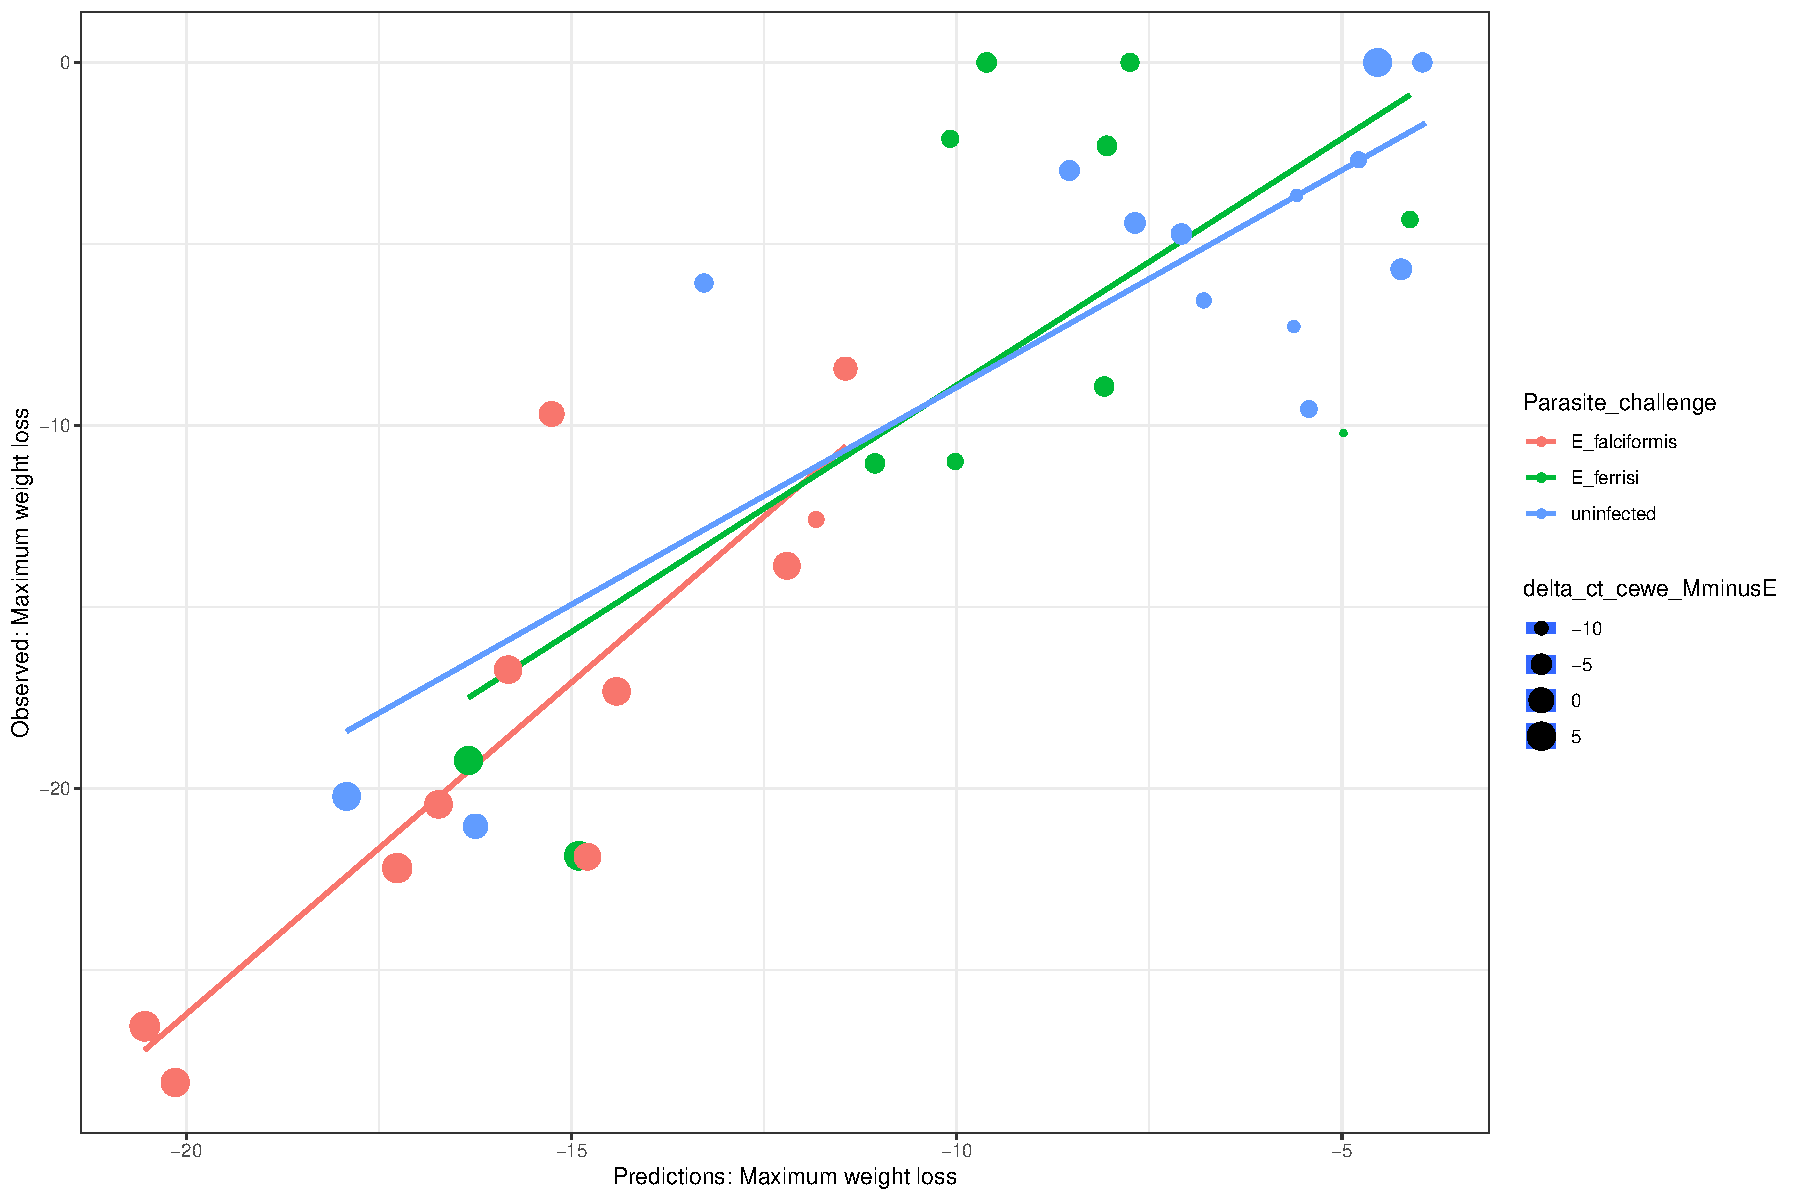
\includegraphics{8.Random_Forest_lab_gene_files/figure-latex/unnamed-chunk-9-1.pdf}

\begin{Shaded}
\begin{Highlighting}[]
\FunctionTok{cor}\NormalTok{(test\_lab}\SpecialCharTok{$}\NormalTok{predictions, test\_lab}\SpecialCharTok{$}\NormalTok{WL\_max, }\AttributeTok{method =} \StringTok{"spearman"}\NormalTok{)}
\end{Highlighting}
\end{Shaded}

\begin{verbatim}
## [1] 0.7995951
\end{verbatim}

\begin{Shaded}
\begin{Highlighting}[]
\NormalTok{test\_lab   }\SpecialCharTok{\%\textgreater{}\%}
  \FunctionTok{ggplot}\NormalTok{(}\FunctionTok{aes}\NormalTok{(}\AttributeTok{x =}\NormalTok{ predictions, }\AttributeTok{y =}\NormalTok{ WL\_max, }\AttributeTok{color =}\NormalTok{ infection, }
                 \AttributeTok{size =}\NormalTok{ delta\_ct\_cewe\_MminusE)) }\SpecialCharTok{+}
  \FunctionTok{geom\_smooth}\NormalTok{(}\AttributeTok{method =}\NormalTok{ lm, }\AttributeTok{se =} \ConstantTok{FALSE}\NormalTok{) }\SpecialCharTok{+}
  \FunctionTok{labs}\NormalTok{(}\AttributeTok{x =} \StringTok{"Predictions: Maximum weight loss"}\NormalTok{, }
       \AttributeTok{y =} \StringTok{"Observed: Maximum weight loss"}\NormalTok{) }\SpecialCharTok{+}
  \FunctionTok{geom\_point}\NormalTok{(}\FunctionTok{aes}\NormalTok{(}\AttributeTok{x =}\NormalTok{ predictions, }\AttributeTok{y =}\NormalTok{ WL\_max, }
                 \AttributeTok{color =}\NormalTok{ infection, }\AttributeTok{size =}\NormalTok{ delta\_ct\_cewe\_MminusE)) }\SpecialCharTok{+}
  \FunctionTok{labs}\NormalTok{(}\AttributeTok{x =} \StringTok{"Predictions: Maximum weight loss"}\NormalTok{, }
       \AttributeTok{y =} \StringTok{"Observed: Maximum weight loss"}\NormalTok{) }\SpecialCharTok{+}
    \FunctionTok{theme\_bw}\NormalTok{()}
\end{Highlighting}
\end{Shaded}

\begin{verbatim}
## `geom_smooth()` using formula 'y ~ x'
\end{verbatim}

\begin{verbatim}
## Warning: Removed 2 rows containing missing values (geom_point).
\end{verbatim}

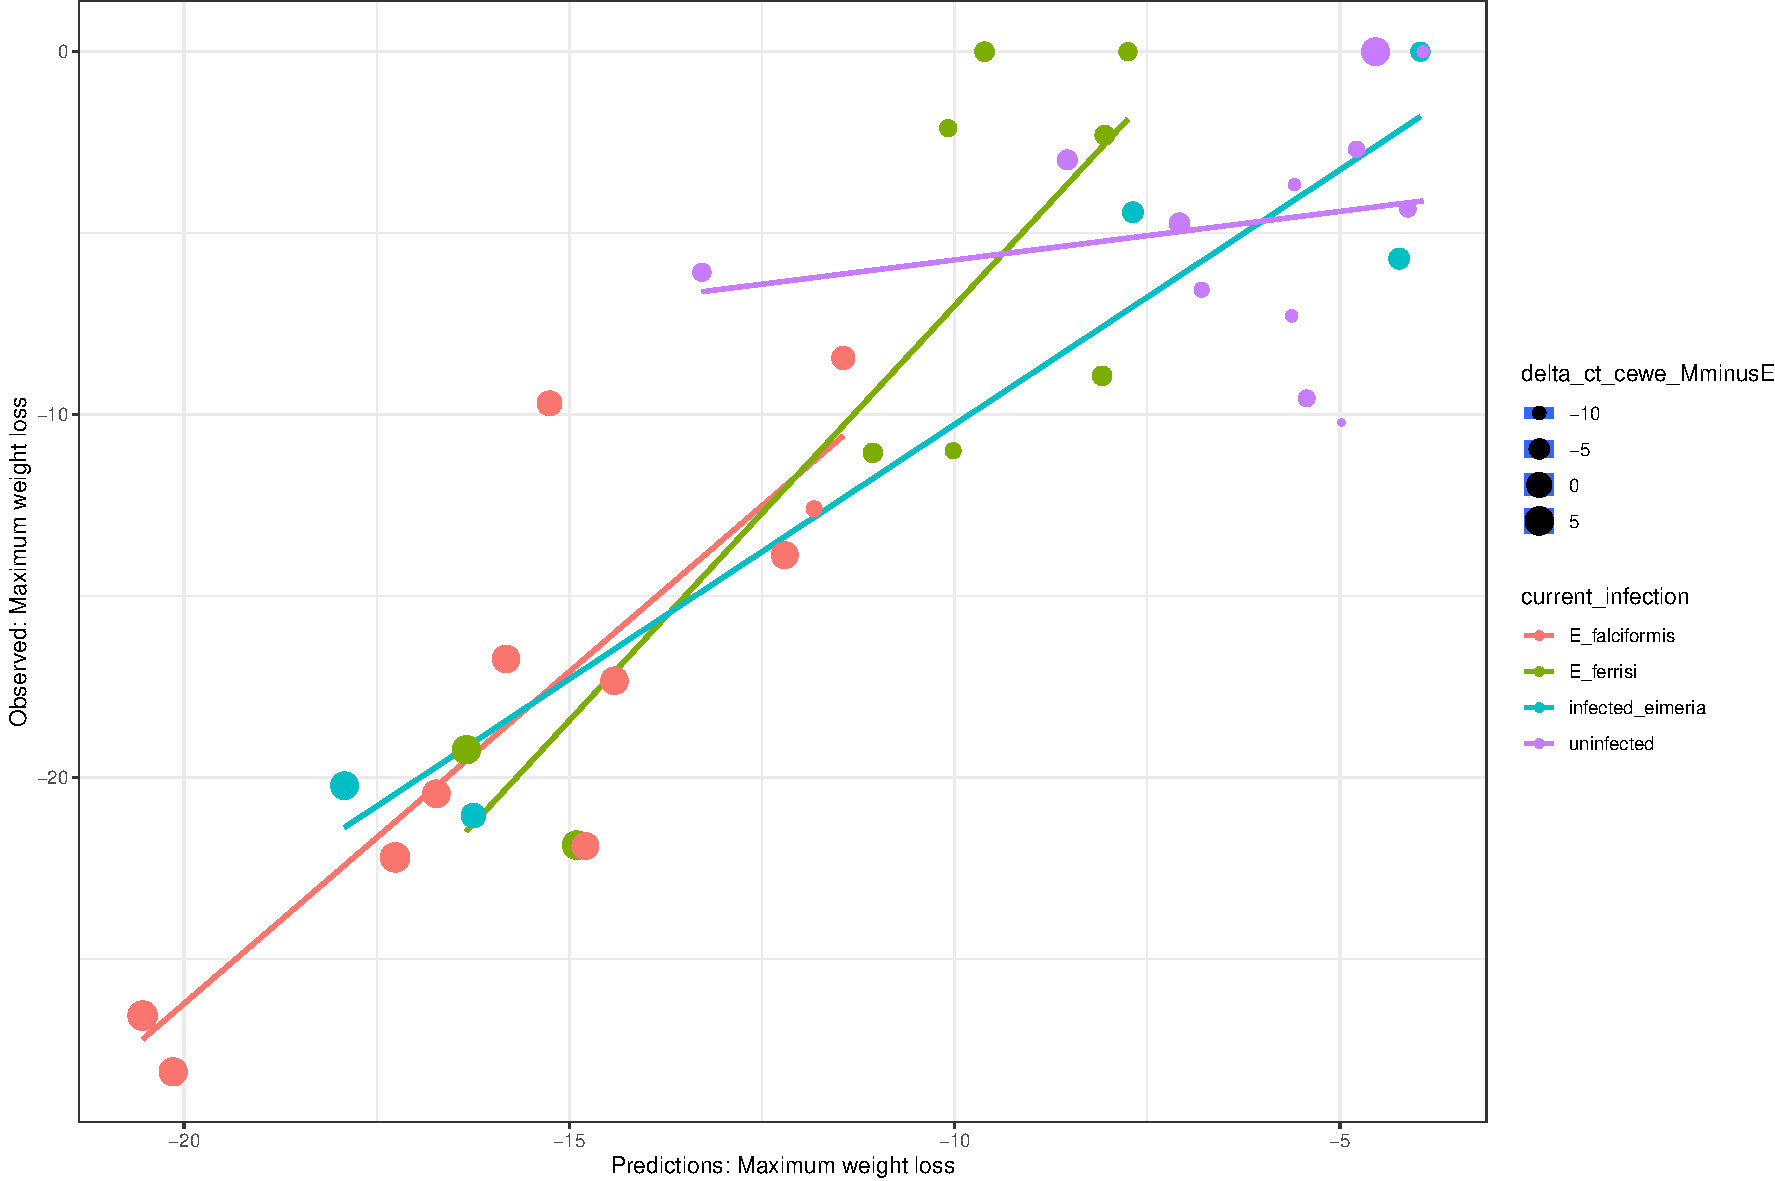
\includegraphics{8.Random_Forest_lab_gene_files/figure-latex/unnamed-chunk-9-2.pdf}

\begin{Shaded}
\begin{Highlighting}[]
\NormalTok{test\_lab   }\SpecialCharTok{\%\textgreater{}\%}
  \FunctionTok{ggplot}\NormalTok{(}\FunctionTok{aes}\NormalTok{(}\AttributeTok{x =}\NormalTok{ predictions, }\AttributeTok{y =}\NormalTok{ WL\_max, }
                 \AttributeTok{size =}\NormalTok{ delta\_ct\_cewe\_MminusE)) }\SpecialCharTok{+}
  \FunctionTok{geom\_smooth}\NormalTok{(}\AttributeTok{method =}\NormalTok{ lm, }\AttributeTok{se =} \ConstantTok{TRUE}\NormalTok{) }\SpecialCharTok{+}
  \FunctionTok{labs}\NormalTok{(}\AttributeTok{x =} \StringTok{"Predictions: Maximum weight loss"}\NormalTok{, }
       \AttributeTok{y =} \StringTok{"Observed: Maximum weight loss"}\NormalTok{) }\SpecialCharTok{+}
  \FunctionTok{geom\_point}\NormalTok{(}\FunctionTok{aes}\NormalTok{(}\AttributeTok{x =}\NormalTok{ predictions, }\AttributeTok{y =}\NormalTok{ WL\_max,  }\AttributeTok{size =}\NormalTok{ delta\_ct\_cewe\_MminusE)) }\SpecialCharTok{+}
  \FunctionTok{labs}\NormalTok{(}\AttributeTok{x =} \StringTok{"Predictions: Maximum weight loss"}\NormalTok{, }
       \AttributeTok{y =} \StringTok{"Observed: Maximum weight loss"}\NormalTok{) }\SpecialCharTok{+}
    \FunctionTok{theme\_bw}\NormalTok{()}
\end{Highlighting}
\end{Shaded}

\begin{verbatim}
## `geom_smooth()` using formula 'y ~ x'
\end{verbatim}

\begin{verbatim}
## Warning: Removed 2 rows containing missing values (geom_point).
\end{verbatim}

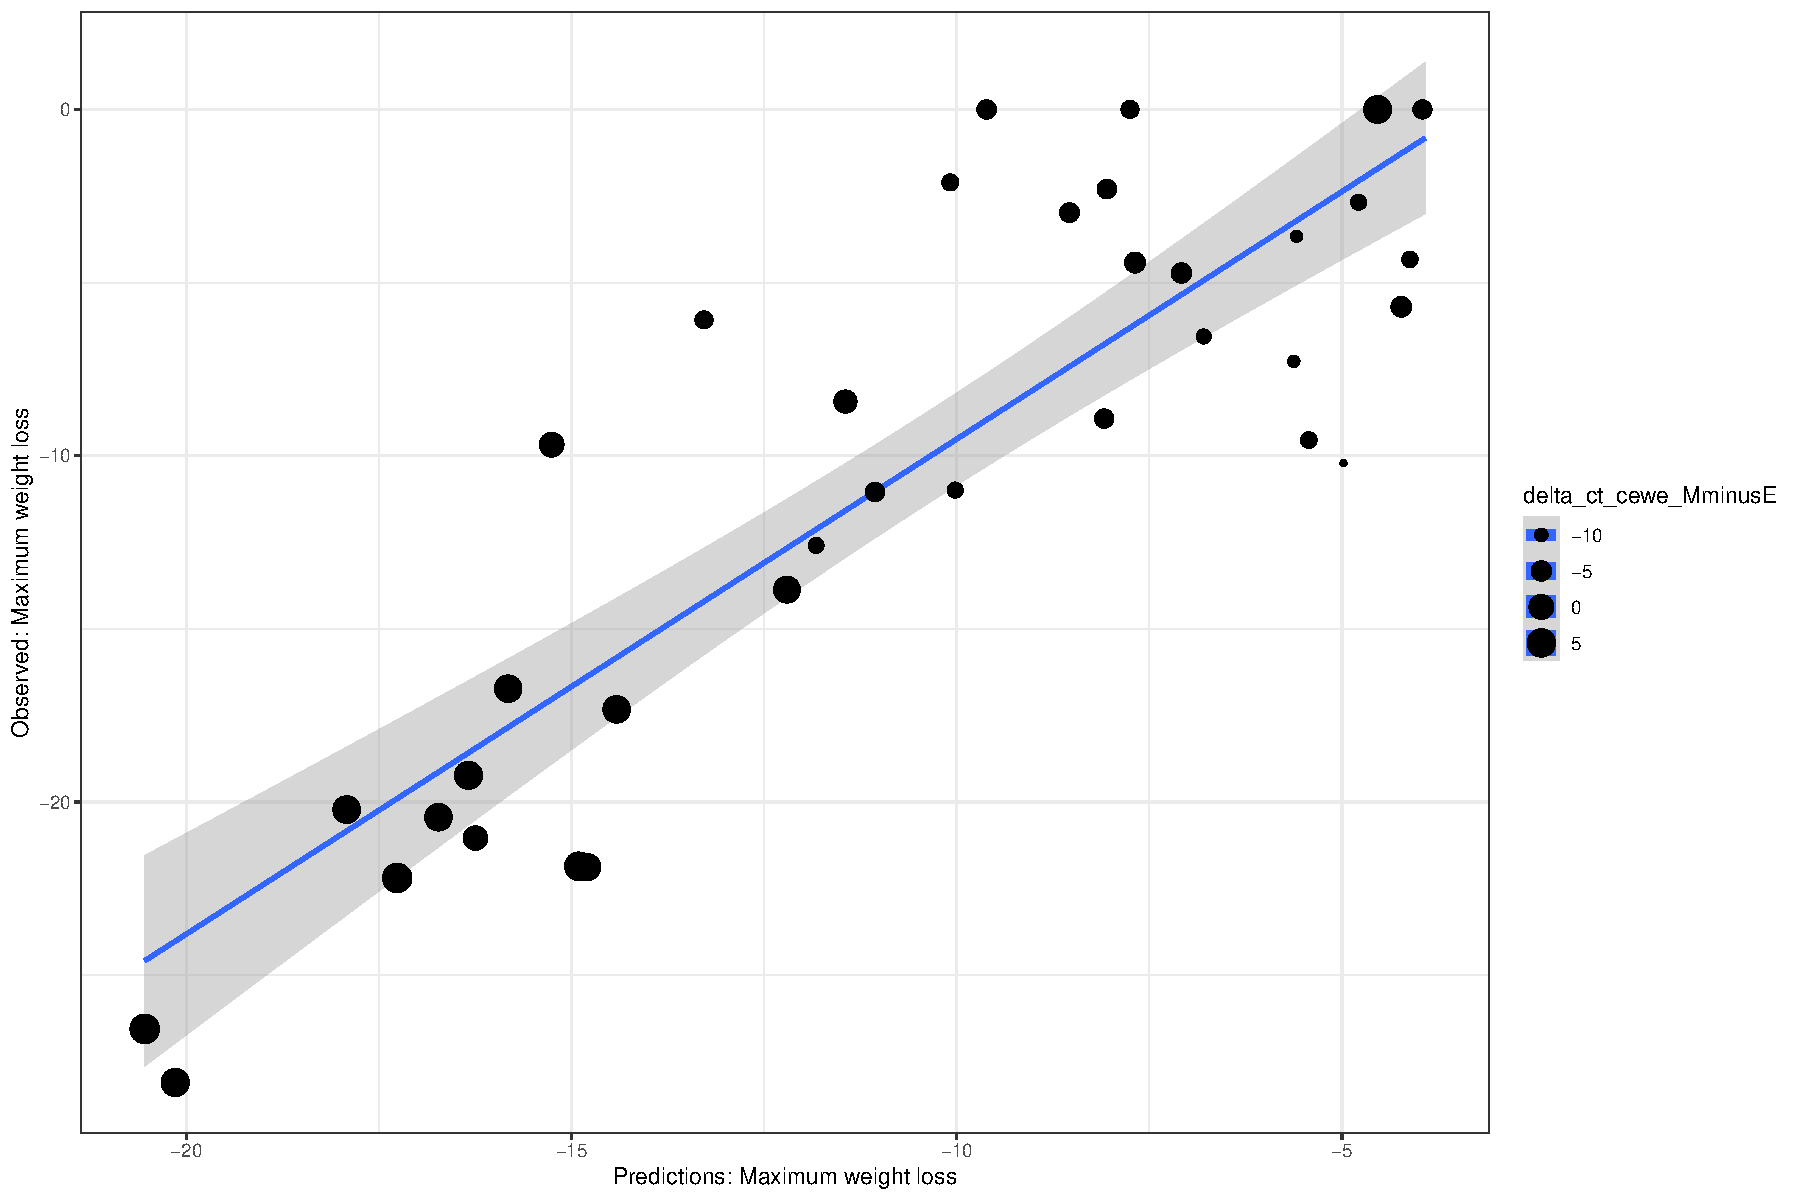
\includegraphics{8.Random_Forest_lab_gene_files/figure-latex/unnamed-chunk-9-3.pdf}
\#\# testing for current infection uninfected + MC positive =
falciformis

\begin{Shaded}
\begin{Highlighting}[]
\CommentTok{\# current\_falciformis}
\CommentTok{\# According to the melting curve for eimeria }
\NormalTok{test\_lab }\OtherTok{\textless{}{-}}\NormalTok{ test\_lab }\SpecialCharTok{\%\textgreater{}\%}
\NormalTok{    dplyr}\SpecialCharTok{::}\FunctionTok{mutate}\NormalTok{(}\AttributeTok{current\_falciformis =} \FunctionTok{case\_when}\NormalTok{(}
\NormalTok{        Parasite\_challenge }\SpecialCharTok{==} \StringTok{"E\_ferrisi"} \SpecialCharTok{\&}\NormalTok{ MC.Eimeria }\SpecialCharTok{==} \StringTok{"TRUE"} \SpecialCharTok{\textasciitilde{}} \StringTok{"E\_ferrisi"}\NormalTok{,}
\NormalTok{        Parasite\_challenge }\SpecialCharTok{==} \StringTok{"E\_ferrisi"} \SpecialCharTok{\&}\NormalTok{ MC.Eimeria }\SpecialCharTok{==} \StringTok{"FALSE"} \SpecialCharTok{\textasciitilde{}} \StringTok{"uninfected"}\NormalTok{,}
\NormalTok{        Parasite\_challenge }\SpecialCharTok{==} \StringTok{"E\_falciformis"} \SpecialCharTok{\&}\NormalTok{ MC.Eimeria }\SpecialCharTok{==} \StringTok{"TRUE"} \SpecialCharTok{\textasciitilde{}} \StringTok{"E\_falciformis"}\NormalTok{,}
\NormalTok{        Parasite\_challenge }\SpecialCharTok{==} \StringTok{"E\_falciformis"} \SpecialCharTok{\&}\NormalTok{ MC.Eimeria }\SpecialCharTok{==} \StringTok{"FALSE"} \SpecialCharTok{\textasciitilde{}} \StringTok{"uninfected"}\NormalTok{,}
\NormalTok{        Parasite\_challenge }\SpecialCharTok{==} \StringTok{"uninfected"} \SpecialCharTok{\&}\NormalTok{ MC.Eimeria }\SpecialCharTok{==} \StringTok{"TRUE"} \SpecialCharTok{\textasciitilde{}} \StringTok{"E\_falciformis"}\NormalTok{,}
\NormalTok{        Parasite\_challenge }\SpecialCharTok{==} \StringTok{"uninfected"} \SpecialCharTok{\&}\NormalTok{ MC.Eimeria }\SpecialCharTok{==} \StringTok{"FALSE"} \SpecialCharTok{\textasciitilde{}} \StringTok{"uninfected"}\NormalTok{,}
        \ConstantTok{TRUE} \SpecialCharTok{\textasciitilde{}} \StringTok{""}
\NormalTok{    ))}

\NormalTok{test\_lab   }\SpecialCharTok{\%\textgreater{}\%}
  \FunctionTok{ggplot}\NormalTok{(}\FunctionTok{aes}\NormalTok{(}\AttributeTok{x =}\NormalTok{ predictions, }\AttributeTok{y =}\NormalTok{ WL\_max, }\AttributeTok{color =}\NormalTok{ current\_falciformis, }
                 \AttributeTok{size =}\NormalTok{ delta\_ct\_cewe\_MminusE)) }\SpecialCharTok{+}
  \FunctionTok{geom\_smooth}\NormalTok{(}\AttributeTok{method =}\NormalTok{ lm, }\AttributeTok{se =} \ConstantTok{FALSE}\NormalTok{) }\SpecialCharTok{+}
  \FunctionTok{labs}\NormalTok{(}\AttributeTok{x =} \StringTok{"Predictions: Maximum weight loss"}\NormalTok{, }
       \AttributeTok{y =} \StringTok{"Observed: Maximum weight loss"}\NormalTok{) }\SpecialCharTok{+}
  \FunctionTok{geom\_point}\NormalTok{(}\FunctionTok{aes}\NormalTok{(}\AttributeTok{x =}\NormalTok{ predictions, }\AttributeTok{y =}\NormalTok{ WL\_max, }
                 \AttributeTok{color =}\NormalTok{ current\_falciformis, }\AttributeTok{size =}\NormalTok{ delta\_ct\_cewe\_MminusE)) }\SpecialCharTok{+}
  \FunctionTok{labs}\NormalTok{(}\AttributeTok{x =} \StringTok{"Predictions: Maximum weight loss"}\NormalTok{, }
       \AttributeTok{y =} \StringTok{"Observed: Maximum weight loss"}\NormalTok{) }\SpecialCharTok{+}
    \FunctionTok{theme\_bw}\NormalTok{()}
\end{Highlighting}
\end{Shaded}

\begin{verbatim}
## `geom_smooth()` using formula 'y ~ x'
\end{verbatim}

\begin{verbatim}
## Warning: Removed 2 rows containing missing values (geom_point).
\end{verbatim}

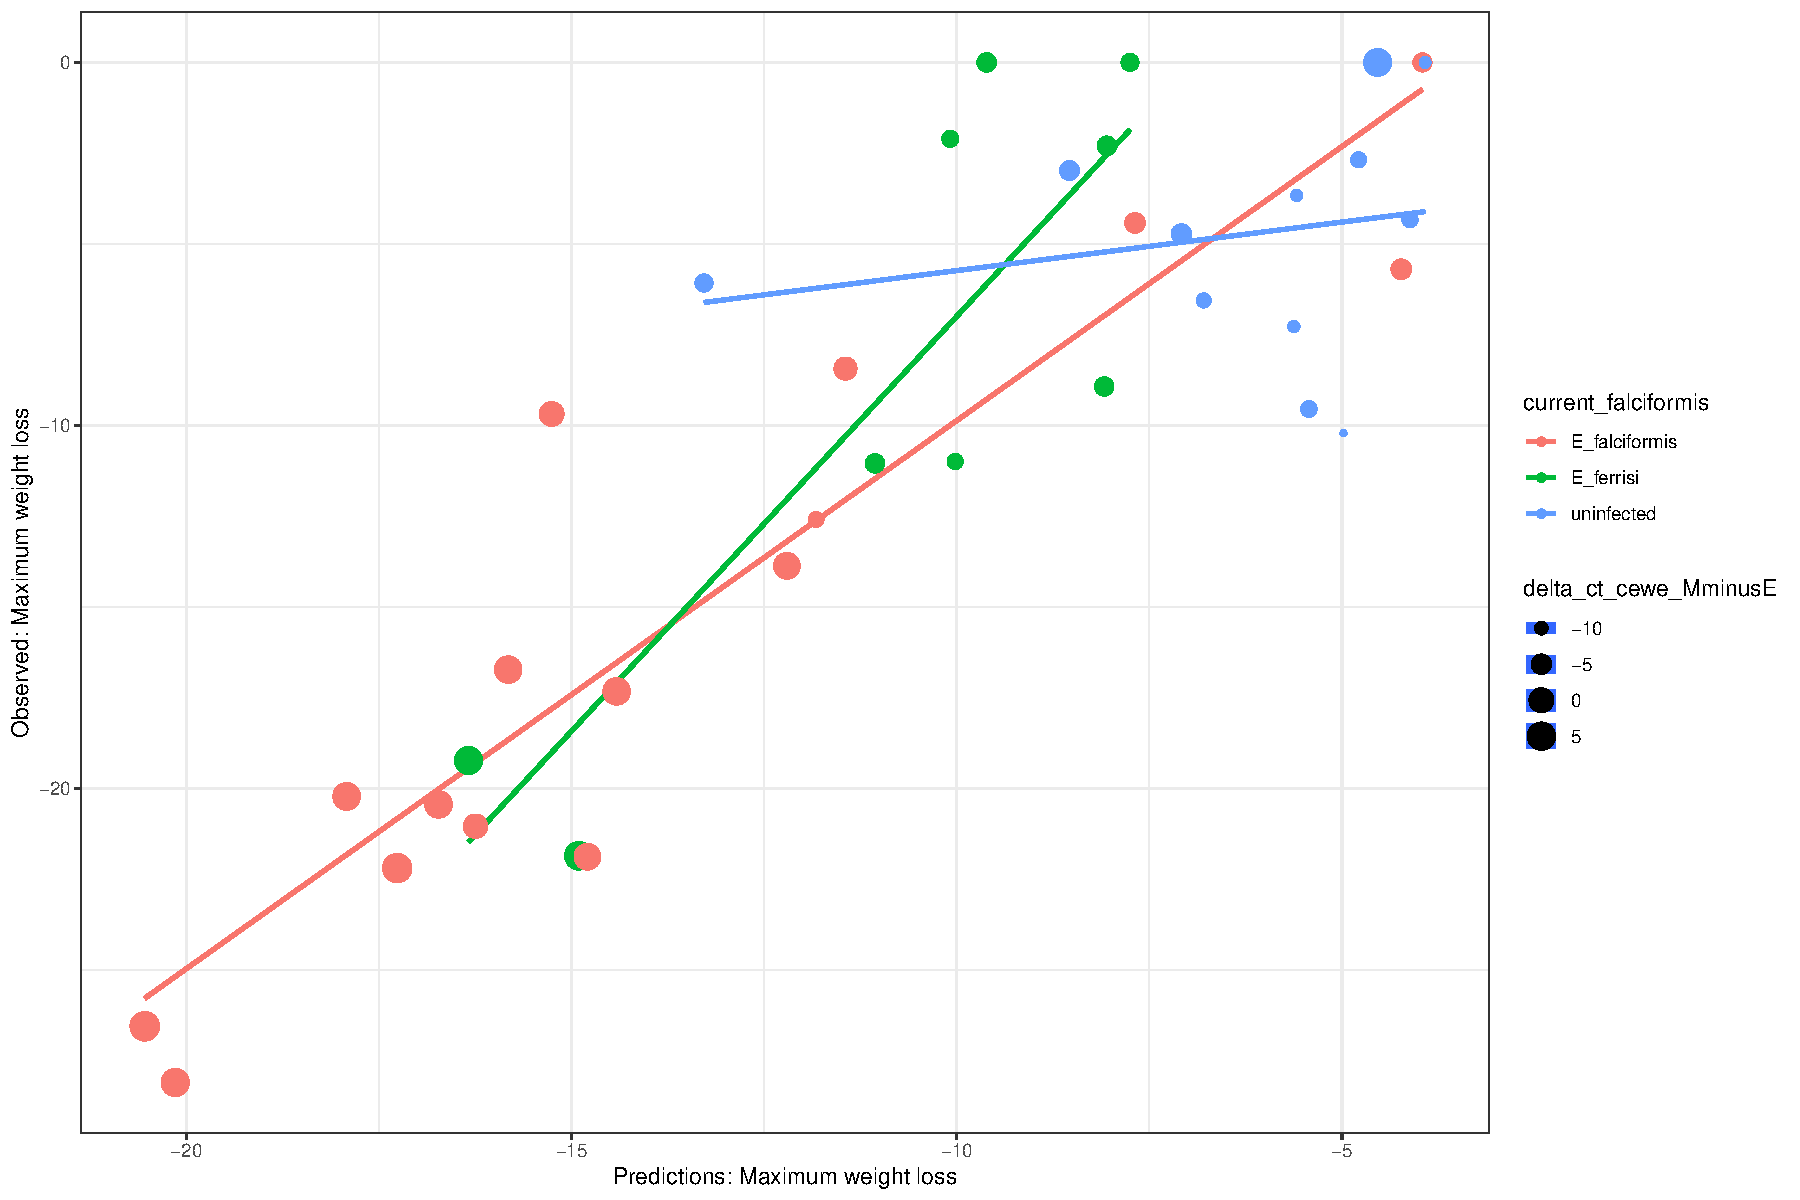
\includegraphics{8.Random_Forest_lab_gene_files/figure-latex/unnamed-chunk-10-1.pdf}

\hypertarget{repeating-the-process-using-the-whole-data-set-as-a-training-data-set}{%
\section{Repeating the process using the whole data set as a training
data
set}\label{repeating-the-process-using-the-whole-data-set-as-a-training-data-set}}

\hypertarget{building-the-model-1}{%
\subsection{Building the model}\label{building-the-model-1}}

\begin{Shaded}
\begin{Highlighting}[]
\CommentTok{\#train the model}
\NormalTok{WL\_predict\_gene }\OtherTok{\textless{}{-}} \FunctionTok{randomForest}\NormalTok{(WL\_max }\SpecialCharTok{\textasciitilde{}}\NormalTok{., }\AttributeTok{data =}\NormalTok{ gene, }
                                    \AttributeTok{proximity =} \ConstantTok{TRUE}\NormalTok{, }\AttributeTok{ntree =} \DecValTok{1000}\NormalTok{) }
\CommentTok{\# ntree = number of trees     }
\CommentTok{\# save the model }
\CommentTok{\# toa = trained on all}
\FunctionTok{saveRDS}\NormalTok{(WL\_predict\_gene, }\StringTok{"r\_scripts/models/predict\_WL.rds"}\NormalTok{)}

\FunctionTok{print}\NormalTok{(WL\_predict\_gene)}
\end{Highlighting}
\end{Shaded}

\begin{verbatim}
## 
## Call:
##  randomForest(formula = WL_max ~ ., data = gene, proximity = TRUE,      ntree = 1000) 
##                Type of random forest: regression
##                      Number of trees: 1000
## No. of variables tried at each split: 6
## 
##           Mean of squared residuals: 28.97269
##                     % Var explained: 53.47
\end{verbatim}

other models

\hypertarget{predicing-parasite-splliting-into-training-and-testing}{%
\subsubsection{Predicing parasite: splliting into training and
testing}\label{predicing-parasite-splliting-into-training-and-testing}}

\begin{Shaded}
\begin{Highlighting}[]
\NormalTok{lab}\SpecialCharTok{$}\NormalTok{Parasite\_challenge }\OtherTok{\textless{}{-}} \FunctionTok{as.factor}\NormalTok{(lab}\SpecialCharTok{$}\NormalTok{Parasite\_challenge)}

\NormalTok{gene\_curr }\OtherTok{\textless{}{-}}\NormalTok{ lab }\SpecialCharTok{\%\textgreater{}\%}
\NormalTok{  dplyr}\SpecialCharTok{::}\FunctionTok{select}\NormalTok{(}\FunctionTok{c}\NormalTok{(Mouse\_ID, }\FunctionTok{all\_of}\NormalTok{(Gene\_lab), Parasite\_challenge))}



\NormalTok{gene }\OtherTok{\textless{}{-}}\NormalTok{ gene\_curr }\SpecialCharTok{\%\textgreater{}\%}
\NormalTok{  dplyr}\SpecialCharTok{::}\FunctionTok{select}\NormalTok{(}\SpecialCharTok{{-}}\NormalTok{Mouse\_ID)}


\CommentTok{\# split data into training and test}
\FunctionTok{set.seed}\NormalTok{(}\DecValTok{123}\NormalTok{) }\CommentTok{\# this will help us reproduce this random assignment}
\CommentTok{\# in this way we can pick the random numbers}
\NormalTok{training.samples }\OtherTok{\textless{}{-}}\NormalTok{ gene}\SpecialCharTok{$}\NormalTok{Parasite\_challenge}\SpecialCharTok{\%\textgreater{}\%}
  \FunctionTok{createDataPartition}\NormalTok{(}\AttributeTok{p =}\NormalTok{ .}\DecValTok{7}\NormalTok{, }\AttributeTok{list =} \ConstantTok{FALSE}\NormalTok{) }
\NormalTok{train.data\_parasite }\OtherTok{\textless{}{-}}\NormalTok{ gene[training.samples, ] }
\NormalTok{test.data\_parasite }\OtherTok{\textless{}{-}}\NormalTok{ gene[}\SpecialCharTok{{-}}\NormalTok{training.samples, ] }
\end{Highlighting}
\end{Shaded}

\#removing infections with falciformis, as we have very few infections
and make our model unreliable

\hypertarget{predicing-parasite-splliting-into-training-and-testing-1}{%
\subsubsection{Predicing parasite: splliting into training and
testing}\label{predicing-parasite-splliting-into-training-and-testing-1}}

\begin{Shaded}
\begin{Highlighting}[]
\NormalTok{lab2 }\OtherTok{\textless{}{-}}\NormalTok{ lab }\SpecialCharTok{\%\textgreater{}\%} 
\NormalTok{  dplyr}\SpecialCharTok{::}\FunctionTok{filter}\NormalTok{(infection }\SpecialCharTok{\%in\%} \FunctionTok{c}\NormalTok{(}\StringTok{"E\_ferrisi"}\NormalTok{, }\StringTok{"uninfected"}\NormalTok{))}


\NormalTok{lab2}\SpecialCharTok{$}\NormalTok{infection }\OtherTok{\textless{}{-}} \FunctionTok{as.factor}\NormalTok{(lab2}\SpecialCharTok{$}\NormalTok{infection)}

\NormalTok{gene\_curr }\OtherTok{\textless{}{-}}\NormalTok{ lab2 }\SpecialCharTok{\%\textgreater{}\%}
\NormalTok{  dplyr}\SpecialCharTok{::}\FunctionTok{select}\NormalTok{(}\FunctionTok{c}\NormalTok{(Mouse\_ID, }\FunctionTok{all\_of}\NormalTok{(Gene\_lab), infection))}



\NormalTok{gene }\OtherTok{\textless{}{-}}\NormalTok{ gene\_curr }\SpecialCharTok{\%\textgreater{}\%}
\NormalTok{  dplyr}\SpecialCharTok{::}\FunctionTok{select}\NormalTok{(}\SpecialCharTok{{-}}\NormalTok{Mouse\_ID)}


\CommentTok{\# split data into training and test}
\FunctionTok{set.seed}\NormalTok{(}\DecValTok{123}\NormalTok{) }\CommentTok{\# this will help us reproduce this random assignment}
\CommentTok{\# in this way we can pick the random numbers}
\NormalTok{training.samples }\OtherTok{\textless{}{-}}\NormalTok{ gene}\SpecialCharTok{$}\NormalTok{infection}\SpecialCharTok{\%\textgreater{}\%}
  \FunctionTok{createDataPartition}\NormalTok{(}\AttributeTok{p =}\NormalTok{ .}\DecValTok{7}\NormalTok{, }\AttributeTok{list =} \ConstantTok{FALSE}\NormalTok{) }
\NormalTok{train.data\_parasite }\OtherTok{\textless{}{-}}\NormalTok{ gene[training.samples, ] }
\NormalTok{test.data\_parasite }\OtherTok{\textless{}{-}}\NormalTok{ gene[}\SpecialCharTok{{-}}\NormalTok{training.samples, ] }
\end{Highlighting}
\end{Shaded}

\hypertarget{building-the-model_parasite}{%
\subsubsection{Building the
model\_Parasite}\label{building-the-model_parasite}}

\begin{Shaded}
\begin{Highlighting}[]
\CommentTok{\#train the model}
\NormalTok{model\_Parasite }\OtherTok{\textless{}{-}} \FunctionTok{randomForest}\NormalTok{(infection }\SpecialCharTok{\textasciitilde{}}\NormalTok{., }
                               \AttributeTok{data =}\NormalTok{ train.data\_parasite, }\AttributeTok{proximity =} \ConstantTok{TRUE}\NormalTok{,}
                      \AttributeTok{ntree =} \DecValTok{1500}\NormalTok{) }\CommentTok{\# number of trees}

\CommentTok{\# save the model }
\FunctionTok{save}\NormalTok{(model\_Parasite, }\AttributeTok{file =}  \StringTok{"r\_scripts/models/predict\_infecting\_parasite.rds"}\NormalTok{)}

\FunctionTok{print}\NormalTok{(model\_Parasite)}
\end{Highlighting}
\end{Shaded}

\begin{verbatim}
## 
## Call:
##  randomForest(formula = infection ~ ., data = train.data_parasite,      proximity = TRUE, ntree = 1500) 
##                Type of random forest: classification
##                      Number of trees: 1500
## No. of variables tried at each split: 4
## 
##         OOB estimate of  error rate: 20.31%
## Confusion matrix:
##            E_ferrisi uninfected class.error
## E_ferrisi         23          8   0.2580645
## uninfected         5         28   0.1515152
\end{verbatim}

\hypertarget{quality-checks}{%
\subsubsection{Quality checks}\label{quality-checks}}

\hypertarget{cross-validation-2}{%
\paragraph{Cross-validation}\label{cross-validation-2}}

MSE: As a brief explanation, mean squared error (MSE) is the average of
the summation of the squared difference between the actual output value
and the predicted output value. Our goal is to reduce the MSE as much as
possible.

Variance explained: \%explained variance is a measure of how well
out-of-bag predictions explain the target variance of the training set.

\begin{Shaded}
\begin{Highlighting}[]
\NormalTok{model\_Parasite\_cv }\OtherTok{\textless{}{-}} \FunctionTok{rf.crossValidation}\NormalTok{(}\AttributeTok{x =}\NormalTok{ model\_Parasite, }\AttributeTok{xdata =}  
\NormalTok{                                          train.data\_parasite, }
                                    \AttributeTok{p =} \FloatTok{0.10}\NormalTok{, }\AttributeTok{n =} \DecValTok{99}\NormalTok{, }\AttributeTok{ntree =} \DecValTok{501}\NormalTok{)}
\end{Highlighting}
\end{Shaded}

\begin{verbatim}
## running: classification cross-validation with 99 iterations
\end{verbatim}

\begin{Shaded}
\begin{Highlighting}[]
\NormalTok{model\_Parasite\_cv}\SpecialCharTok{$}\NormalTok{fit.var.exp}
\end{Highlighting}
\end{Shaded}

\begin{verbatim}
## NULL
\end{verbatim}

\begin{Shaded}
\begin{Highlighting}[]
\CommentTok{\# Plot cross validation versus model producers accuracy}
\end{Highlighting}
\end{Shaded}

\hypertarget{testing-the-model-predictions}{%
\subsubsection{Testing the model:
Predictions}\label{testing-the-model-predictions}}

\begin{Shaded}
\begin{Highlighting}[]
\CommentTok{\#The predict() function in R is used to predict the values based on the input }
\CommentTok{\# data.}
\NormalTok{predictions\_parasite }\OtherTok{\textless{}{-}} \FunctionTok{predict}\NormalTok{(model\_Parasite, test.data\_parasite)}
\CommentTok{\# assign test.data to a new object, so that we can make changes}
\NormalTok{result\_parasite }\OtherTok{\textless{}{-}}\NormalTok{ test.data\_parasite}
\CommentTok{\#add the new variable of predictions to the result object}
\NormalTok{result\_parasite }\OtherTok{\textless{}{-}} \FunctionTok{cbind}\NormalTok{(result\_parasite, predictions\_parasite)}
\CommentTok{\#add the results to a data frame containing test data and the prediction}
\NormalTok{result\_parasite }\OtherTok{\textless{}{-}} \FunctionTok{cbind}\NormalTok{(lab2[}\FunctionTok{row.names}\NormalTok{(result\_parasite), ], predictions\_parasite)}
\end{Highlighting}
\end{Shaded}

\hypertarget{visualizing-predictions_parasite}{%
\subsubsection{Visualizing
predictions\_parasite}\label{visualizing-predictions_parasite}}

\begin{Shaded}
\begin{Highlighting}[]
\NormalTok{conf\_matrix\_parasite }\OtherTok{\textless{}{-}} 
  \FunctionTok{confusionMatrix}\NormalTok{(}
\NormalTok{    result\_parasite}\SpecialCharTok{$}\NormalTok{predictions\_parasite,}
    \AttributeTok{reference =}\NormalTok{ result\_parasite}\SpecialCharTok{$}\NormalTok{infection)}

\FunctionTok{print}\NormalTok{(conf\_matrix\_parasite)}
\end{Highlighting}
\end{Shaded}

\begin{verbatim}
## Confusion Matrix and Statistics
## 
##             Reference
## Prediction   E_ferrisi uninfected
##   E_ferrisi         10          2
##   uninfected         3         12
##                                          
##                Accuracy : 0.8148         
##                  95% CI : (0.6192, 0.937)
##     No Information Rate : 0.5185         
##     P-Value [Acc > NIR] : 0.001421       
##                                          
##                   Kappa : 0.6281         
##                                          
##  Mcnemar's Test P-Value : 1.000000       
##                                          
##             Sensitivity : 0.7692         
##             Specificity : 0.8571         
##          Pos Pred Value : 0.8333         
##          Neg Pred Value : 0.8000         
##              Prevalence : 0.4815         
##          Detection Rate : 0.3704         
##    Detection Prevalence : 0.4444         
##       Balanced Accuracy : 0.8132         
##                                          
##        'Positive' Class : E_ferrisi      
## 
\end{verbatim}

\begin{Shaded}
\begin{Highlighting}[]
\NormalTok{conf\_matrix\_parasite}\SpecialCharTok{$}\NormalTok{table}
\end{Highlighting}
\end{Shaded}

\begin{verbatim}
##             Reference
## Prediction   E_ferrisi uninfected
##   E_ferrisi         10          2
##   uninfected         3         12
\end{verbatim}

\begin{Shaded}
\begin{Highlighting}[]
\NormalTok{plt }\OtherTok{\textless{}{-}} \FunctionTok{as.data.frame}\NormalTok{(conf\_matrix\_parasite}\SpecialCharTok{$}\NormalTok{table)}
\NormalTok{plt}\SpecialCharTok{$}\NormalTok{Prediction }\OtherTok{\textless{}{-}} \FunctionTok{factor}\NormalTok{(plt}\SpecialCharTok{$}\NormalTok{Prediction, }\AttributeTok{levels=}\FunctionTok{rev}\NormalTok{(}\FunctionTok{levels}\NormalTok{(plt}\SpecialCharTok{$}\NormalTok{Prediction)))}

\FunctionTok{ggplot}\NormalTok{(plt, }\FunctionTok{aes}\NormalTok{(}\AttributeTok{x =}\NormalTok{ Prediction, }\AttributeTok{y =}\NormalTok{  Reference, }\AttributeTok{fill=}\NormalTok{ Freq)) }\SpecialCharTok{+}
        \FunctionTok{geom\_tile}\NormalTok{() }\SpecialCharTok{+} \FunctionTok{geom\_text}\NormalTok{(}\FunctionTok{aes}\NormalTok{(}\AttributeTok{label=}\NormalTok{Freq)) }\SpecialCharTok{+}
        \FunctionTok{scale\_fill\_gradient}\NormalTok{(}\AttributeTok{low=}\StringTok{"white"}\NormalTok{, }\AttributeTok{high=}\StringTok{"darkturquoise"}\NormalTok{) }\SpecialCharTok{+}
        \FunctionTok{labs}\NormalTok{(}\AttributeTok{x =} \StringTok{"Predictions"}\NormalTok{,}\AttributeTok{y =} \StringTok{"Reference"}\NormalTok{) }
\end{Highlighting}
\end{Shaded}

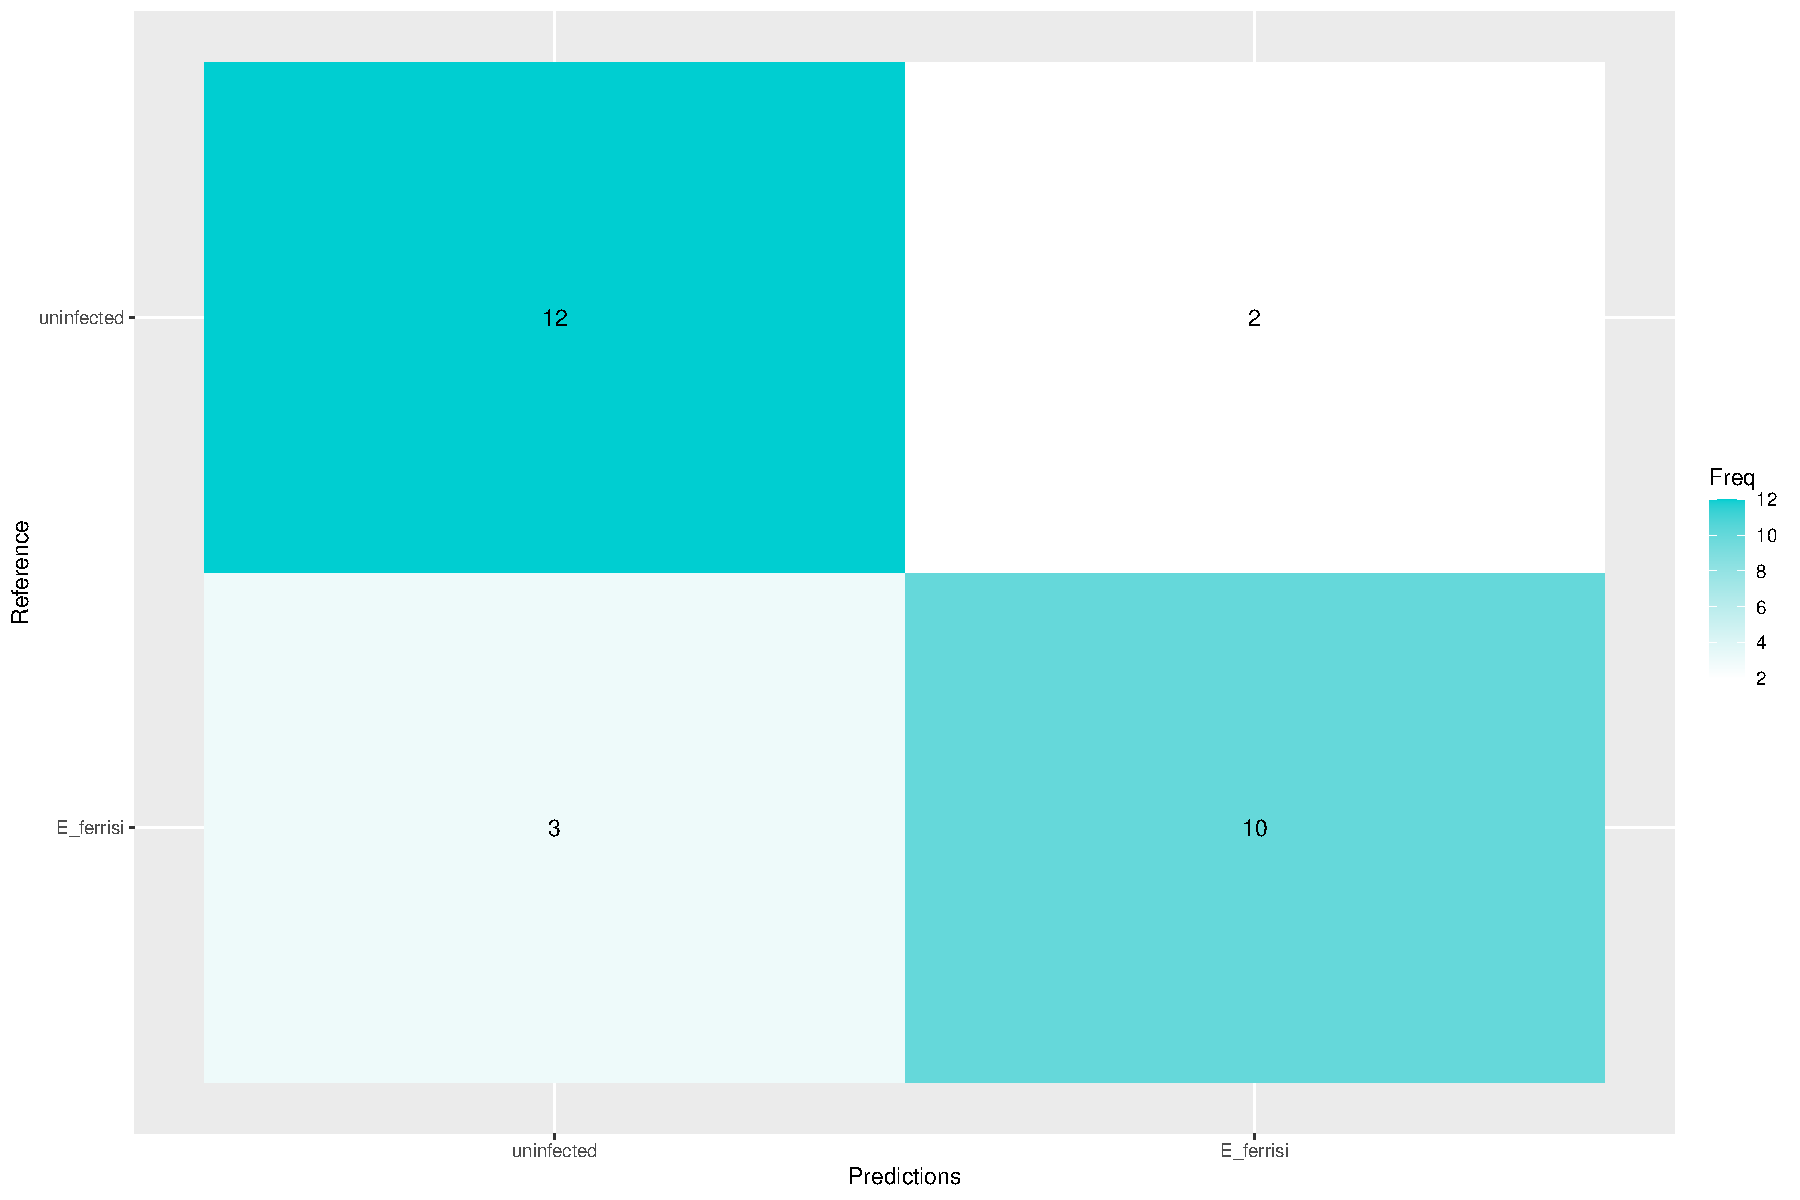
\includegraphics{8.Random_Forest_lab_gene_files/figure-latex/unnamed-chunk-17-1.pdf}

\hypertarget{repeating-the-process-using-the-whole-data-set-as-a-training-data-set-1}{%
\section{Repeating the process using the whole data set as a training
data
set}\label{repeating-the-process-using-the-whole-data-set-as-a-training-data-set-1}}

\hypertarget{building-the-model-2}{%
\subsection{Building the model}\label{building-the-model-2}}

\begin{Shaded}
\begin{Highlighting}[]
\CommentTok{\#train the model}
\NormalTok{model\_Parasite }\OtherTok{\textless{}{-}} \FunctionTok{randomForest}\NormalTok{(infection }\SpecialCharTok{\textasciitilde{}}\NormalTok{., }\AttributeTok{data =}\NormalTok{ gene, }
                                    \AttributeTok{proximity =} \ConstantTok{TRUE}\NormalTok{, }\AttributeTok{ntree =} \DecValTok{1000}\NormalTok{) }
\CommentTok{\# ntree = number of trees     }
\CommentTok{\# save the model }
\CommentTok{\# toa = trained on all}
\FunctionTok{saveRDS}\NormalTok{(model\_Parasite, }\StringTok{"r\_scripts/models/predict\_infecting\_parasite.rds"}\NormalTok{)}

\FunctionTok{print}\NormalTok{(model\_Parasite)}
\end{Highlighting}
\end{Shaded}

\begin{verbatim}
## 
## Call:
##  randomForest(formula = infection ~ ., data = gene, proximity = TRUE,      ntree = 1000) 
##                Type of random forest: classification
##                      Number of trees: 1000
## No. of variables tried at each split: 4
## 
##         OOB estimate of  error rate: 17.58%
## Confusion matrix:
##            E_ferrisi uninfected class.error
## E_ferrisi         35          9   0.2045455
## uninfected         7         40   0.1489362
\end{verbatim}

\hypertarget{predicing-eimeria-mc-splliting-into-training-and-testing}{%
\subsubsection{Predicing Eimeria MC: splliting into training and
testing}\label{predicing-eimeria-mc-splliting-into-training-and-testing}}

\begin{Shaded}
\begin{Highlighting}[]
\FunctionTok{str}\NormalTok{(lab}\SpecialCharTok{$}\NormalTok{MC.Eimeria)}
\end{Highlighting}
\end{Shaded}

\begin{verbatim}
##  Factor w/ 2 levels "FALSE","TRUE": 2 2 1 2 2 2 2 2 2 2 ...
\end{verbatim}

\begin{Shaded}
\begin{Highlighting}[]
\NormalTok{MC }\OtherTok{\textless{}{-}}\NormalTok{ lab }\SpecialCharTok{\%\textgreater{}\%}
\NormalTok{  dplyr}\SpecialCharTok{::}\FunctionTok{select}\NormalTok{(}\FunctionTok{c}\NormalTok{(Mouse\_ID, }\FunctionTok{all\_of}\NormalTok{(Gene\_lab), MC.Eimeria))}



\NormalTok{MC }\OtherTok{\textless{}{-}}\NormalTok{ MC }\SpecialCharTok{\%\textgreater{}\%}
\NormalTok{  dplyr}\SpecialCharTok{::}\FunctionTok{select}\NormalTok{(}\SpecialCharTok{{-}}\NormalTok{Mouse\_ID)}


\CommentTok{\# split data into training and test}
\FunctionTok{set.seed}\NormalTok{(}\DecValTok{182}\NormalTok{) }\CommentTok{\# this will help us reproduce this random assignment}
\CommentTok{\# in this way we can pick the random numbers}
\NormalTok{training.samples }\OtherTok{\textless{}{-}}\NormalTok{ MC}\SpecialCharTok{$}\NormalTok{MC.Eimeria }\SpecialCharTok{\%\textgreater{}\%}
  \FunctionTok{createDataPartition}\NormalTok{(}\AttributeTok{p =}\NormalTok{ .}\DecValTok{7}\NormalTok{, }\AttributeTok{list =} \ConstantTok{FALSE}\NormalTok{) }

\NormalTok{train.data\_MC }\OtherTok{\textless{}{-}}\NormalTok{ MC[training.samples, ] }
\NormalTok{test.data\_MC }\OtherTok{\textless{}{-}}\NormalTok{ MC[}\SpecialCharTok{{-}}\NormalTok{training.samples, ] }
\end{Highlighting}
\end{Shaded}

\hypertarget{building-the-model_mc}{%
\subsubsection{Building the model\_MC}\label{building-the-model_mc}}

\begin{Shaded}
\begin{Highlighting}[]
\CommentTok{\#train the model}
\NormalTok{model\_MC }\OtherTok{\textless{}{-}} \FunctionTok{randomForest}\NormalTok{(MC.Eimeria }\SpecialCharTok{\textasciitilde{}}\NormalTok{., }
                               \AttributeTok{data =}\NormalTok{ train.data\_MC, }\AttributeTok{proximity =} \ConstantTok{TRUE}\NormalTok{,}
                      \AttributeTok{ntree =} \DecValTok{1500}\NormalTok{) }\CommentTok{\# number of trees}

\CommentTok{\# save the model }
\FunctionTok{saveRDS}\NormalTok{(model\_MC, }\AttributeTok{file =}  \StringTok{"r\_scripts/models/predict\_MC.rds"}\NormalTok{)}

\FunctionTok{print}\NormalTok{(model\_MC)}
\end{Highlighting}
\end{Shaded}

\begin{verbatim}
## 
## Call:
##  randomForest(formula = MC.Eimeria ~ ., data = train.data_MC,      proximity = TRUE, ntree = 1500) 
##                Type of random forest: classification
##                      Number of trees: 1500
## No. of variables tried at each split: 4
## 
##         OOB estimate of  error rate: 18.95%
## Confusion matrix:
##       FALSE TRUE class.error
## FALSE    24    9   0.2727273
## TRUE      9   53   0.1451613
\end{verbatim}

\hypertarget{quality-checks-1}{%
\subsubsection{Quality checks}\label{quality-checks-1}}

\hypertarget{cross-validation-3}{%
\paragraph{Cross-validation}\label{cross-validation-3}}

MSE: As a brief explanation, mean squared error (MSE) is the average of
the summation of the squared difference between the actual output value
and the predicted output value. Our goal is to reduce the MSE as much as
possible.

Variance explained: \%explained variance is a measure of how well
out-of-bag predictions explain the target variance of the training set.

\begin{Shaded}
\begin{Highlighting}[]
\NormalTok{model\_MC\_cv }\OtherTok{\textless{}{-}} \FunctionTok{rf.crossValidation}\NormalTok{(}\AttributeTok{x =}\NormalTok{ model\_MC, }\AttributeTok{xdata =}  
\NormalTok{                                          train.data\_MC, }
                                    \AttributeTok{p =} \FloatTok{0.10}\NormalTok{, }\AttributeTok{n =} \DecValTok{99}\NormalTok{, }\AttributeTok{ntree =} \DecValTok{501}\NormalTok{)}
\end{Highlighting}
\end{Shaded}

\begin{verbatim}
## running: classification cross-validation with 99 iterations
\end{verbatim}

\begin{Shaded}
\begin{Highlighting}[]
\NormalTok{model\_MC\_cv}\SpecialCharTok{$}\NormalTok{fit.var.exp}
\end{Highlighting}
\end{Shaded}

\begin{verbatim}
## NULL
\end{verbatim}

\begin{Shaded}
\begin{Highlighting}[]
\CommentTok{\# Plot cross validation versus model producers accuracy}
\end{Highlighting}
\end{Shaded}

\hypertarget{testing-the-model-predictions-1}{%
\subsubsection{Testing the model:
Predictions}\label{testing-the-model-predictions-1}}

\begin{Shaded}
\begin{Highlighting}[]
\CommentTok{\#The predict() function in R is used to predict the values based on the input }
\CommentTok{\# data.}
\NormalTok{predictions\_MC }\OtherTok{\textless{}{-}} \FunctionTok{predict}\NormalTok{(model\_MC, test.data\_MC)}

\CommentTok{\# assign test.data to a new object, so that we can make changes}
\NormalTok{result\_MC }\OtherTok{\textless{}{-}}\NormalTok{ test.data\_MC}
\CommentTok{\#add the new variable of predictions to the result object}
\NormalTok{result\_MC }\OtherTok{\textless{}{-}} \FunctionTok{cbind}\NormalTok{(result\_MC, predictions\_MC)}
\CommentTok{\#add the results to a data frame containing test data and the prediction}
\NormalTok{result\_MC }\OtherTok{\textless{}{-}} \FunctionTok{cbind}\NormalTok{(lab[}\FunctionTok{row.names}\NormalTok{(result\_MC), ], predictions\_MC)}
\end{Highlighting}
\end{Shaded}

\hypertarget{visualizing-predictions_mc}{%
\subsubsection{Visualizing
predictions\_MC}\label{visualizing-predictions_mc}}

\begin{Shaded}
\begin{Highlighting}[]
\NormalTok{conf\_matrix\_MC }\OtherTok{\textless{}{-}} 
  \FunctionTok{confusionMatrix}\NormalTok{(result\_MC}\SpecialCharTok{$}\NormalTok{predictions\_MC, }\AttributeTok{reference =}\NormalTok{ result\_MC}\SpecialCharTok{$}\NormalTok{MC.Eimeria)}

\FunctionTok{print}\NormalTok{(conf\_matrix\_MC)}
\end{Highlighting}
\end{Shaded}

\begin{verbatim}
## Confusion Matrix and Statistics
## 
##           Reference
## Prediction FALSE TRUE
##      FALSE     9    8
##      TRUE      5   18
##                                           
##                Accuracy : 0.675           
##                  95% CI : (0.5087, 0.8143)
##     No Information Rate : 0.65            
##     P-Value [Acc > NIR] : 0.4408          
##                                           
##                   Kappa : 0.3194          
##                                           
##  Mcnemar's Test P-Value : 0.5791          
##                                           
##             Sensitivity : 0.6429          
##             Specificity : 0.6923          
##          Pos Pred Value : 0.5294          
##          Neg Pred Value : 0.7826          
##              Prevalence : 0.3500          
##          Detection Rate : 0.2250          
##    Detection Prevalence : 0.4250          
##       Balanced Accuracy : 0.6676          
##                                           
##        'Positive' Class : FALSE           
## 
\end{verbatim}

\begin{Shaded}
\begin{Highlighting}[]
\NormalTok{conf\_matrix\_MC}\SpecialCharTok{$}\NormalTok{table}
\end{Highlighting}
\end{Shaded}

\begin{verbatim}
##           Reference
## Prediction FALSE TRUE
##      FALSE     9    8
##      TRUE      5   18
\end{verbatim}

\begin{Shaded}
\begin{Highlighting}[]
\NormalTok{plt }\OtherTok{\textless{}{-}} \FunctionTok{as.data.frame}\NormalTok{(conf\_matrix\_MC}\SpecialCharTok{$}\NormalTok{table)}
\NormalTok{plt}\SpecialCharTok{$}\NormalTok{Prediction }\OtherTok{\textless{}{-}} \FunctionTok{factor}\NormalTok{(plt}\SpecialCharTok{$}\NormalTok{Prediction, }\AttributeTok{levels=}\FunctionTok{rev}\NormalTok{(}\FunctionTok{levels}\NormalTok{(plt}\SpecialCharTok{$}\NormalTok{Prediction)))}

\FunctionTok{ggplot}\NormalTok{(plt, }\FunctionTok{aes}\NormalTok{(}\AttributeTok{x =}\NormalTok{ Prediction, }\AttributeTok{y =}\NormalTok{  Reference, }\AttributeTok{fill=}\NormalTok{ Freq)) }\SpecialCharTok{+}
        \FunctionTok{geom\_tile}\NormalTok{() }\SpecialCharTok{+} \FunctionTok{geom\_text}\NormalTok{(}\FunctionTok{aes}\NormalTok{(}\AttributeTok{label=}\NormalTok{Freq)) }\SpecialCharTok{+}
        \FunctionTok{scale\_fill\_gradient}\NormalTok{(}\AttributeTok{low=}\StringTok{"white"}\NormalTok{, }\AttributeTok{high=}\StringTok{"darkturquoise"}\NormalTok{) }\SpecialCharTok{+}
        \FunctionTok{labs}\NormalTok{(}\AttributeTok{x =} \StringTok{"Predictions"}\NormalTok{,}\AttributeTok{y =} \StringTok{"Reference"}\NormalTok{) }
\end{Highlighting}
\end{Shaded}

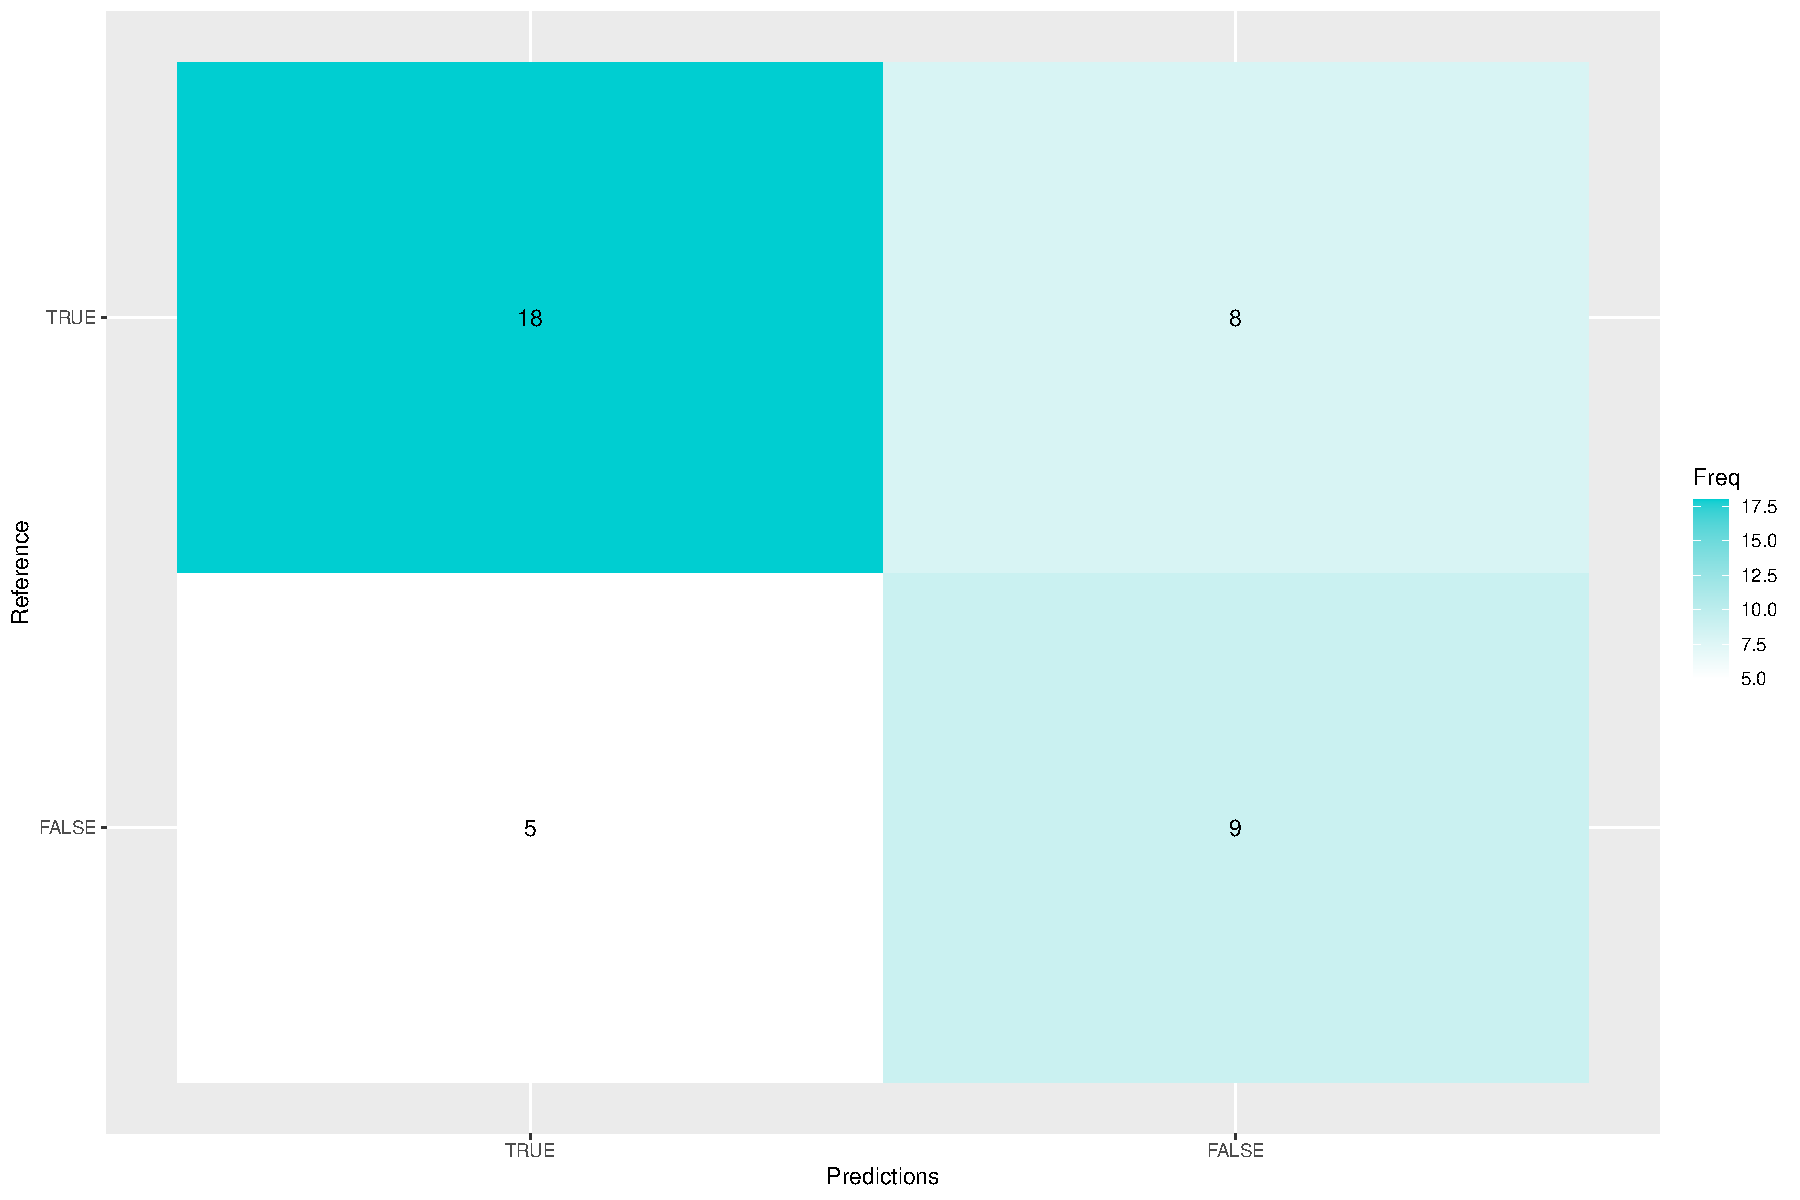
\includegraphics{8.Random_Forest_lab_gene_files/figure-latex/unnamed-chunk-23-1.pdf}

\end{document}
